% ===================================================
\section{Problem Statement}
% ===================================================
In this chapter, we consider a two-agent pursuit-evasion problem that involves  a Target (aircraft) in opposition to an Attacker (missile). The Target tries to evade the Attacker and avoid being captured by him. We will try to find a simple technique for target evasion, so we should have a look at evasion techniques.

\subsection{Evasion techniques}
There is some observations we should make before talking about evasion techniques 
\begin{itemize}
	\item The missile is faster than the aircraft, but cannot turn tighter than the aircraft, so it takes a longer path.
	\item The control mechanism of the Missile is much simpler and is of less capability than that of the aircraft. In order to pull as tight turn as the aircraft, it must exercise an acceleration that is far beyond its capability.
	\item The missile always attempts to trace the target. Thus if the target changes heading, it will necessary for the Missile to change heading similarly, but this is too difficult for him to achieve.
	\item  The main problem with evading missiles is their speed, which makes timing somewhat difficult.
\end{itemize}

%\begin{table}
%	\begin{tabular}{ |c|c|c|c| } 
%		\hline  %-----------------------
%   If missile is fired head-on at BVR range
% & Jinking (useful at short ranges) 
% & Climb (useful at longer ranges)
% & Fourth tactic \\
%%		\hline  %---------------
%		\hline  %---------------
%		
% Turn hard to either left or right so as to fly at roughly 90 degrees angle to attacking aircraft (This forces missile to bleed off the energy and to lead the target).
% Once target aircraft makes a hard turn to reverse a direction, missile with its far larger turn circle – will be unable to compensate.
%	
%		 &  %||||||||||
%		
% Aircraft must be positioned so that it is at angle (30-60 degrees is optimum) relative to missile’s flight path.
% Once missile gets closer, aircraft will make a hard turn in opposite direction.
%As there is a lag between aircraft changing the direction and missile following (for several reasons, most important of which is missile’s inertia), this will cause missile to head in wrong direction until it manages to correct, and also to bleed off the energy
% Missile will fly past the aircraft and miss.
%	
%	 &   %|||||||||||||
%	 
%	 
% Since at long range missile will have burned out its engine, it will rely on inertia to keep it flying, and climbing will mean that it will bleed off energy rapidly.
% Once missile reaches a close range (maybe around 1,500 meters), dive for the ground, then pull up (This will allow pilot to gain energy and using it to evade the missile).
%	 
%	  &    %|||||||||||
%	   
% place the missile at 3 o’clock or 9 o’clock position
% maintain sufficient turn to keep the missile 
% This tactic forces the missile to execute a continuous turn, bleeding the energy entire time, making it easier to outturn the missile once it comes close.
%	   \\
	%		\hline  %------------------------------- 
	%		 \begin{figure}[htb]
	%		 	\centering
	%		 	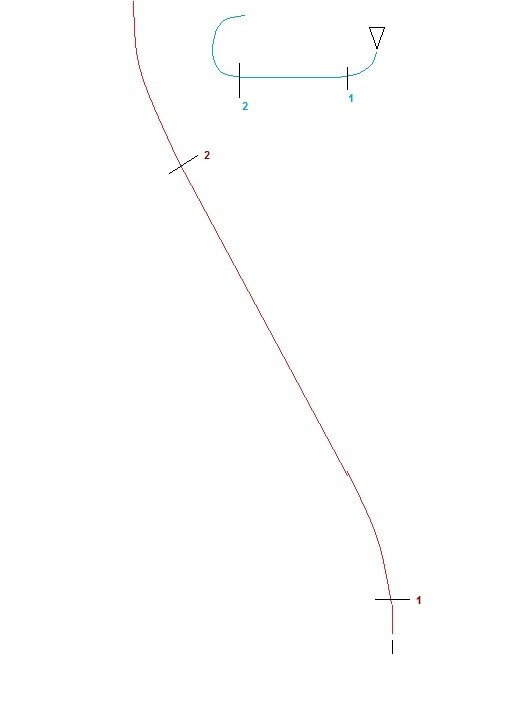
\includegraphics[scale = 0.3]{fig/evasion tech1.jpg}
	%		 \end{figure}
	
	% & %||||||||||||||||||||
	 
	%	\begin{figure}[htb]
	%		 \centering
	%		 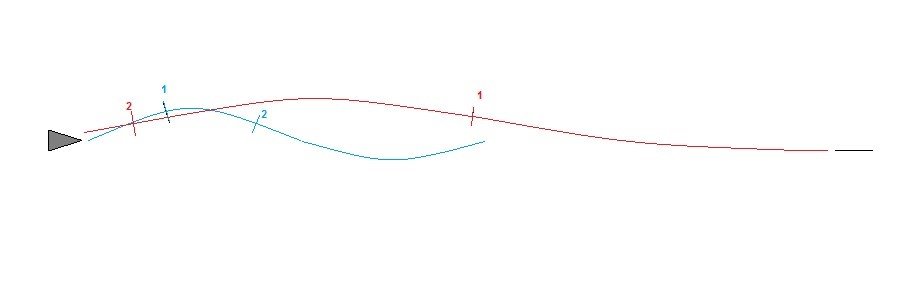
\includegraphics[scale = 0.3]{fig/evasion tech2.jpg}
	%	\end{figure} 
	
	%    &    %|||||||||||||||||
	
	%\begin{figure}[htb]
	%	\centering
	%	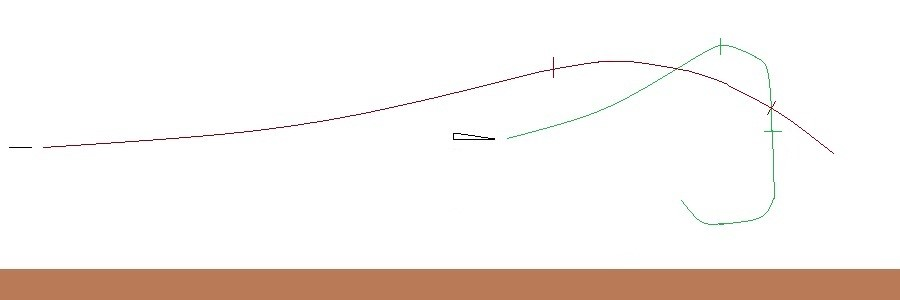
\includegraphics[scale = 0.3]{fig/evasion tech3.jpg}
	%\end{figure}
	
	
	%    &    %||||||||||||||||||| 
	 
	 
	%\begin{figure}[htb]
	%\centering
	%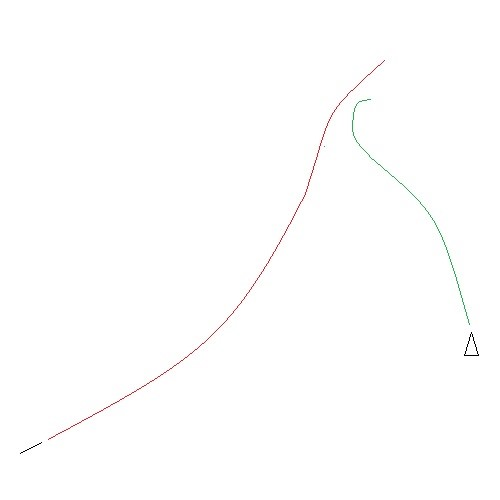
\includegraphics[scale = 0.3]{fig/evasion tech4.jpg}
	%\end{figure}\\
	%		\hline   %----------------
	
	
	%	\end{tabular}
	%	\caption{A variety of evasion techniques}
	%	\label{evasion tech}
	%\end{table}  



%Why use polynomials?
Now we want to search for a path that the Target can move on it to escape from the Attacker. All the evasion techniques depend on the time of the turn that the Target makes when it detects the Attacker (Missile) and the objective is to maximize the Missile acceleration till the Missile power bleed. 
We will  choose the escaping trajectory as a polynomial with unknown coefficients, then try to find these coefficients which make the Missile exert a maximum acceleration to bleed its power as fast as we can before it reaches the Target.  
% ===================================================
\section{Assumptions, Notation, and Nomenclature}
% ===================================================
\subsection*{Assumptions}

\begin{enumerate}
	\item Both the Attacker and Target travel at constant speeds.
	\item The Attacker's speed is larger than that of the Target. Otherwise, the Target will be unconditionally or trivially capable of escaping. 
	\item Gravitational and drag effects are neglected for simplicity.
\end{enumerate}
% ===================================================

% ===================================================
\subsection*{Notation}
% ===================================================
\begin{itemize}
	\item $n_c$ : Acceleration command (for the Missile) in $m/s^2$.
	\item $N'$ : Effective navigation ratio, a unit-less designer-chosen gain (usually in the range of $3\to5$).
	\item $V_c$ : Missile-Target closing velocity.
	\item $\lambda$ : line-of-sight angle.
	\item $\dot{\lambda}$ : line of sight rate.
	\item $R_{TM}$ : length of the line of sight.
	\item $L$ : Missile lead angle.
	\item $HE$ : Heading error.
	\item $\dot{\beta}$ : angular velocity of the Target.
	\item $V_{T1},V_{T2}$ : Target velocity components in the Earth fixed coordinate system.
	\item $V_{M1},V_{M2}$ : Missile velocity components in the Earth fixed coordinate system.
\end{itemize}
% ===================================================
\subsection*{Nomenclature}

\textbf{Inertial coordinate system:} fixed to the surface of a flat-Earth model ( the 1 axis is downrange and the 2 axis can either be altitude or cross-range).

\textbf{Missile lead angle:} theoretically correct angle
for the missile to be on a collision triangle with the Target.

\textbf{Heading error ($HE$) :} angle representing the initial deviation of the Missile from the collision triangle.

\textbf{line of sight:} The imaginary line connecting the Missile and Target.

\textbf{length of the line of sight ($R_{TM}$):} Instantaneous separation between Missile and Target.

\textbf{Miss distance :} The point of closest approach of the Missile and Target.

\textbf{Closing velocity ($V_c$):} the negative rate of change of the distance
from the Missile to the Target $Vc= -\dot{R_{TM}}=-\frac{d}{dt} R_{TM} $.


% ===================================================


% ===================================================
\section{Proportional Navigation}
% ===================================================
In this section, we will illustrate some fundamentals of missile guidance, focusing on the proportional navigation technique, which is one of the simplest guidance laws.

\subsection*{What is proportional navigation?}
The proportional navigation guidance law issues acceleration commands,
perpendicular to the instantaneous missile-target line-of-sight, which are
proportional to the line-of-sight rate and closing velocity. Mathematically, the
guidance law can be stated as

\begin{equation}
	n_c= N' V_c \dot{\lambda}
	\label{PNeq}
\end{equation}

where $n_c$ is the acceleration command (for the missile) in $(m/s^2)$, $N'$ is the the effective navigation ratio, a unit-less designer-chosen gain (usually in the range of $3 \to 5$), $V_c$ is the missile-target closing velocity in $(m/s)$ and $\dot{\lambda} = \frac{d\lambda}{dt}$ is the rate of the line-of-sight angle and is in $(rad/s)$. Note that (\ref{PNeq}) is dimensionally homogeneous, since $n_c$ has the dimension
\begin{equation}
	\begin{split}
	[n_c] &= [N'] [V_c] [\dot{\lambda}]\\
	&=(1) (LT^-1) (T^-1)\\
	&=LT^-2
	\end{split}
	\label{PN dimensionallity}
\end{equation}
which is the appropriate dimension of linear acceleration.

\subsection{Simulation of proportional navigation equations in 2-D}
In this subsection we will introduce the equations of proportional navigation and the sequence to get a simulation for the path of the Target and the Attacker and how the missile acceleration will be affected during this simulation.

\textbf{The simulation inputs} are the initial location of the Missile ($R_{M1}, R_{M2}$) and the initial location of the Target ($R_{T1}, R_{T2}$), Target speed $V_T$, Missile speed $V_M$, and effective navigation ratio $N'$.

There are two types of \textbf{error sources} that cause the Attacker to miss the Target; they are the heading error ($HE$) and the acceleration of the Target ($n_T$) called the Target maneuver.

\begin{figure}[htb]
	\centering
	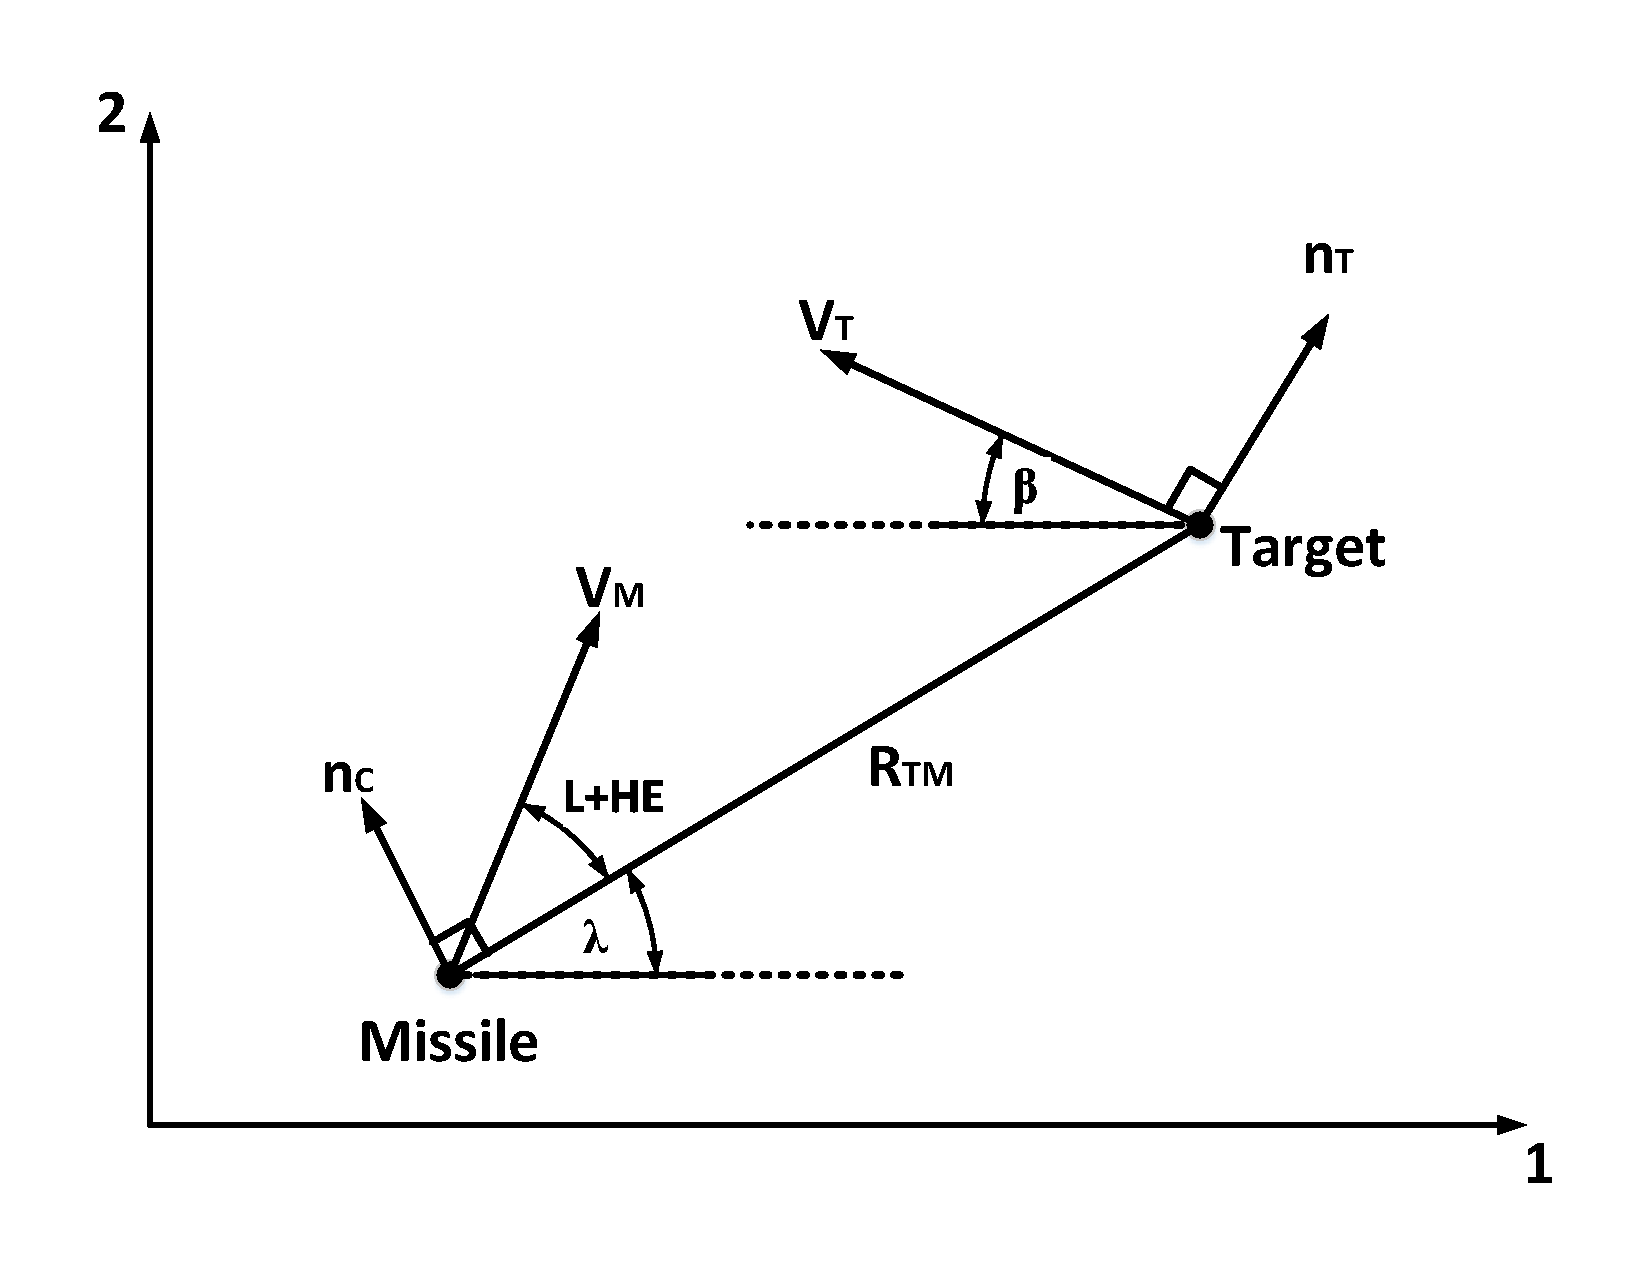
\includegraphics[scale = 0.65]{fig/PN.pdf}
	\caption{Two dimensional Missile-Target engagement geometry.}
	\label{PN}
\end{figure}


\subsubsection*{proportional navigation differential equations}

\textbf{The components of Target velocity} 
\begin{equation}
	V_{T1} = - V_T \cos(\beta)
\end{equation}

\begin{equation}
V_{T2} =  V_T \sin(\beta)
\end{equation}

\textbf{Relative missile-target separation}
\begin{equation}
	R_{TM1} = R{T1} - R_{M1}
\end{equation}
\begin{equation}
R_{TM2} = R{T2} - R_{M2}
\end{equation}

from the previous 2 equations we get
\begin{equation}
	R_{TM} = \sqrt{R_{TM1}^2 + R_{TM2}^2}
	\label{RTM}
\end{equation}

\textbf{line of sight angle}
\begin{equation}
	\lambda = \tan^{-1} (\dfrac{R_{TM2}}{R_{TM1}})
	\label{lambda}
\end{equation}

\textbf{missile lead angle} 
\begin{equation}
	L= \sin^{-1}(\dfrac{V_T \sin(\beta + \lambda)}{V_M})
\end{equation}

the angle between the downrange axis and $V_M$ vector is $\theta = \lambda + L$

\textbf{Missile velocity components} 

\begin{equation}
	V_{M1} = V_M \cos (\theta + HE)
\end{equation}

\begin{equation}
V_{M2} = V_M \sin (\theta + HE)
\end{equation}

\textbf{Relative velocity components}
\begin{equation}
	V_{TM1} = V_{T1} - V_{M1}
\end{equation}

\begin{equation}
V_{TM2} = V_{T2} - V_{M12}
\end{equation}


\textbf{closing velocity} it is the negative rate of change of the distance
from the missile to the target $Vc= -R_{TM} $, so we have to differentiate eq(\ref{RTM})

\begin{center}
	$\dot{R_{TM}}= \frac{1}{2} (R_{TM1}^2 + R_{TM2}^2)^{\frac{-1}{2}} [2 R_{TM1} \dot{R_{TM1}} + 2 R_{TM2} \dot{R_{TM2}}]$
\end{center}

we see that
%\begin{equation*}
% \dot{R_{TM1}=V_{TM1} , \dot{R_{TM2}=V_{TM2}
%\end{equation*}
%and 
%\begin{equation*}
%(R_{TM1}^2 + R_{TM2}^2)^{\frac{-1}{2}} = \dfrac{1}{R_{TM}}
%\end{equation*}
so we get 
\begin{equation}
	V_c = - \dot{R_{TM}} = - \dfrac{R_{TM1} V_{TM1}+R_{TM2} V_{TM2}}{R_{TM}}
\end{equation}

\textbf{line of sight rate} we have to differentiate eq(\ref{lambda}) using the rule $\tan^{-1}x = \frac{dx}{1+x^2}$ 

\begin{equation}
	\begin{split}
	\dot{\lambda} &= [\dfrac{1}{1+(\frac{R_{TM2}}{R_{TM1}})^2}] \dot{(\frac{R_{TM2}}{R_{TM1}})}\\
	&= \dfrac{R_{TM1}^2}{R_{TM1}^2 + R_{TM2}^2}[\dfrac{R_{TM1}\dot{R_{TM2}}- R_{TM2} \dot{R_{TM1}}}{R_{TM1}^2}]\\
	&=\dfrac{R_{TM1} V_{TM2} - R_{TM2} V_{TM1}}{R_{TM1}^2}
	\end{split}
\end{equation}

\textbf{magnitude of the missile guidance command}
\begin{equation}
		n_c= N' V_c \dot{\lambda}
\end{equation}

\textbf{missile acceleration components}
\begin{equation}
	a_{M1} = - n_c \sin \lambda
\end{equation}

\begin{equation}
a_{M2} = - n_c \cos \lambda
\end{equation}

\textbf{angular velocity of the target}
\begin{equation}
	\dot{\beta} = \dfrac{n_T}{V_T}
\end{equation}

we will solve all the equations in this section using second-order Runge-Kutta numerical integration procedure. If we have a first order differential equation of the form 
\begin{equation*}
	\dot{x} = f(x,t) 
\end{equation*} 
 where t is time, we seek to find a recursive relationship for x as a function of time.
 With the second-order Runge–Kutta numerical technique, the value of x at the
 next integration interval h is given by
 \begin{equation*}
 	x_{k+1} = x_k + \dfrac{hf(x,t)}{2} + \dfrac{h f(x, t+h)}{2}
 \end{equation*}
% ===================================================
\section{Models \& Simulations}
% ===================================================

In this section we will simulate equations in sec. 2.3 for proportional navigation using MATLAB and Simulink.
The following figure is a flowchart illustrating the steps of calculations using the equations in sec. 2.3  till we plot the trajectories.

\begin{figure}[htb]
	\centering
	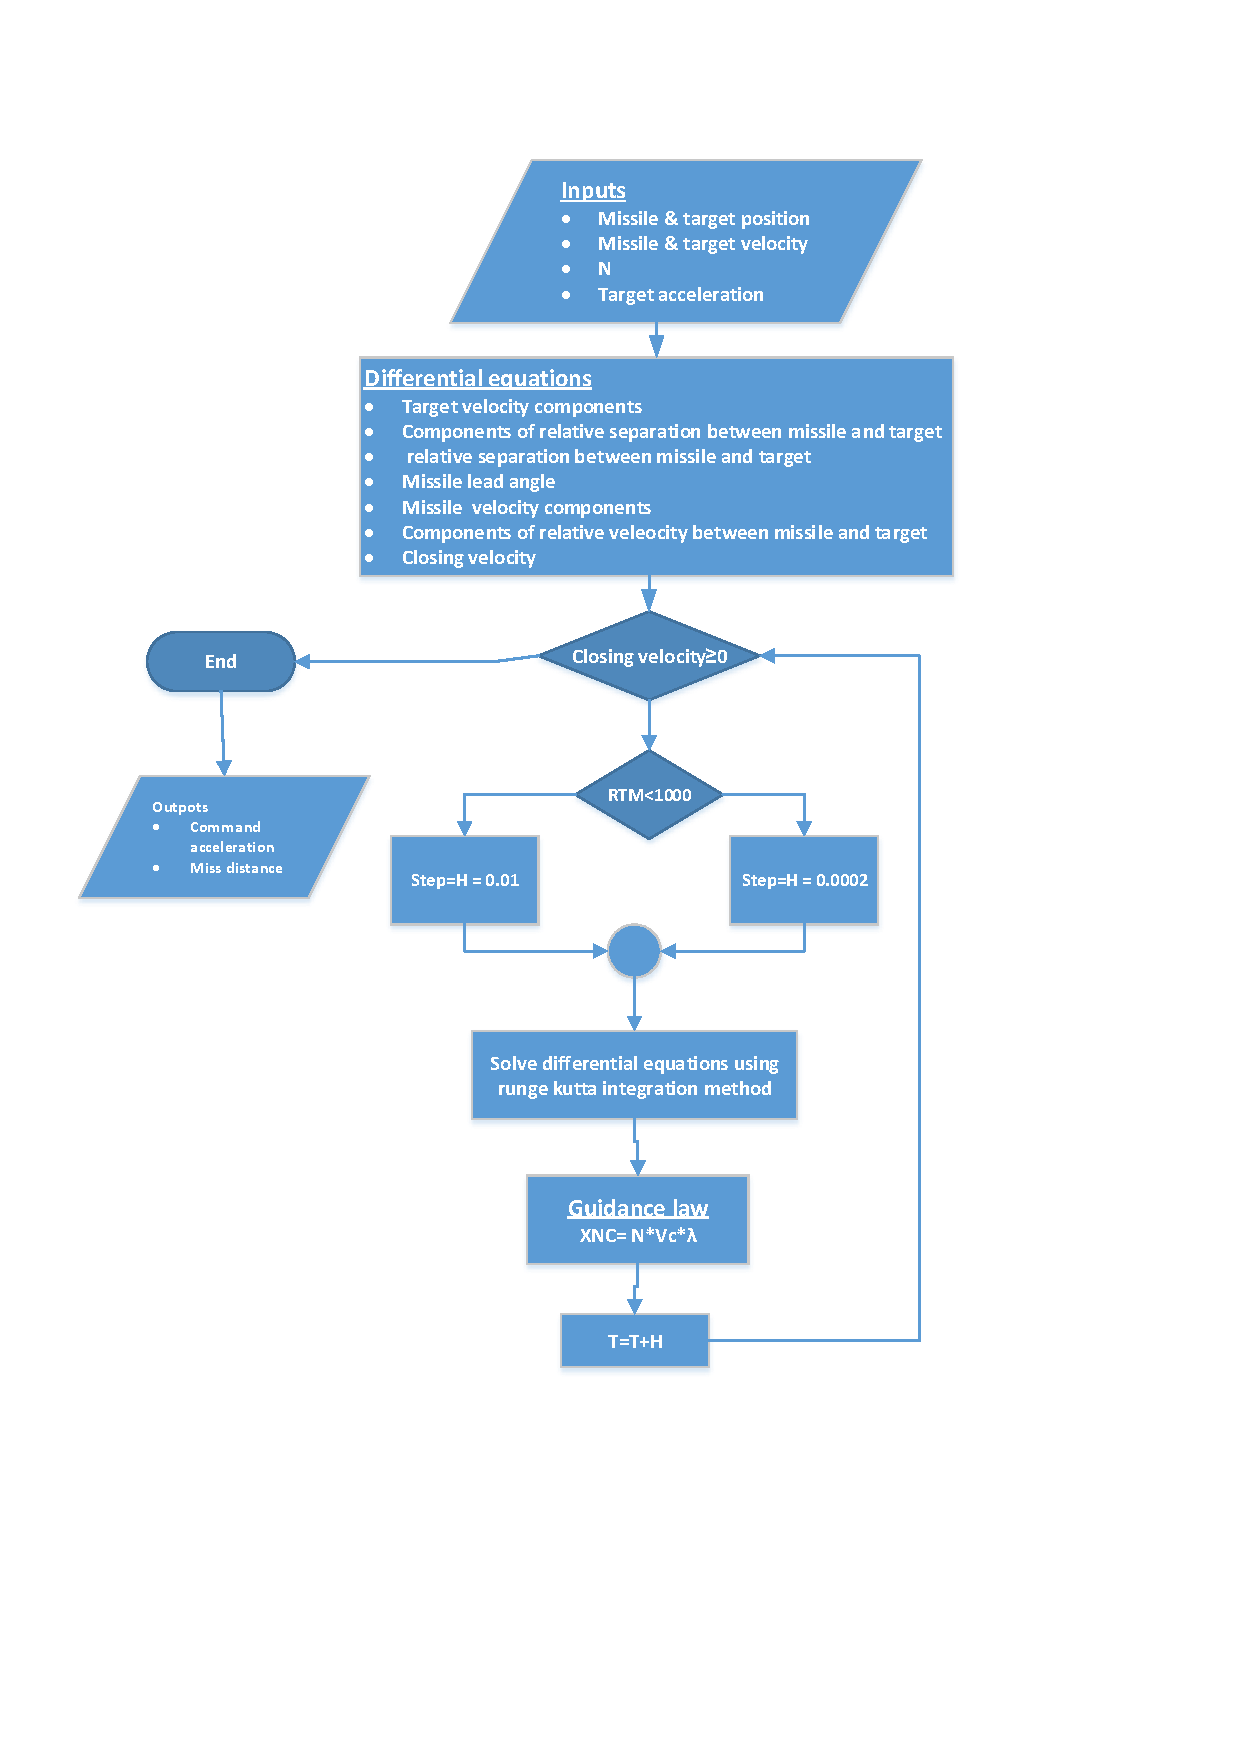
\includegraphics[scale = 0.85]{fig/FlowchartPN.pdf}
	\caption{Flowchart illustrating the steps of calculations using the equations in sec. 2.3  till we plot the trajectories.}
	\label{flowchart PN}
\end{figure}


\subsection{MATLAB}
In this subsection we will use MATLAB to simulate equations in sec. 2.3 for proportional navigation. We will solve the differential equations using second-order Runge-Kutta numerical integration technique, then we will draw the trajectories of the pursuit and evader for 4 cases for the Target maneuver error source, and we will deduce the effect of the effective navigation ratio $N'$ and the other type of the error source; Heading error. 
\subsubsection{Zero Target maneuver}
In this case the evader (Target - plane) does not do any effort to scape, it just moves in a straight line, as we see in Fig. \ref{trajectory0N4}. So the pursuer (Attacker - Missile) does not have to bleed much energy to reach the Target.

In the case of \textbf{zero Heading error} the effective navigation ratio has no effect on the simulation engagement at all. The missile's acceleration will be zero as in Fig. \ref{missile acceleration0N4}.

\begin{figure}[htb]
	\centering
	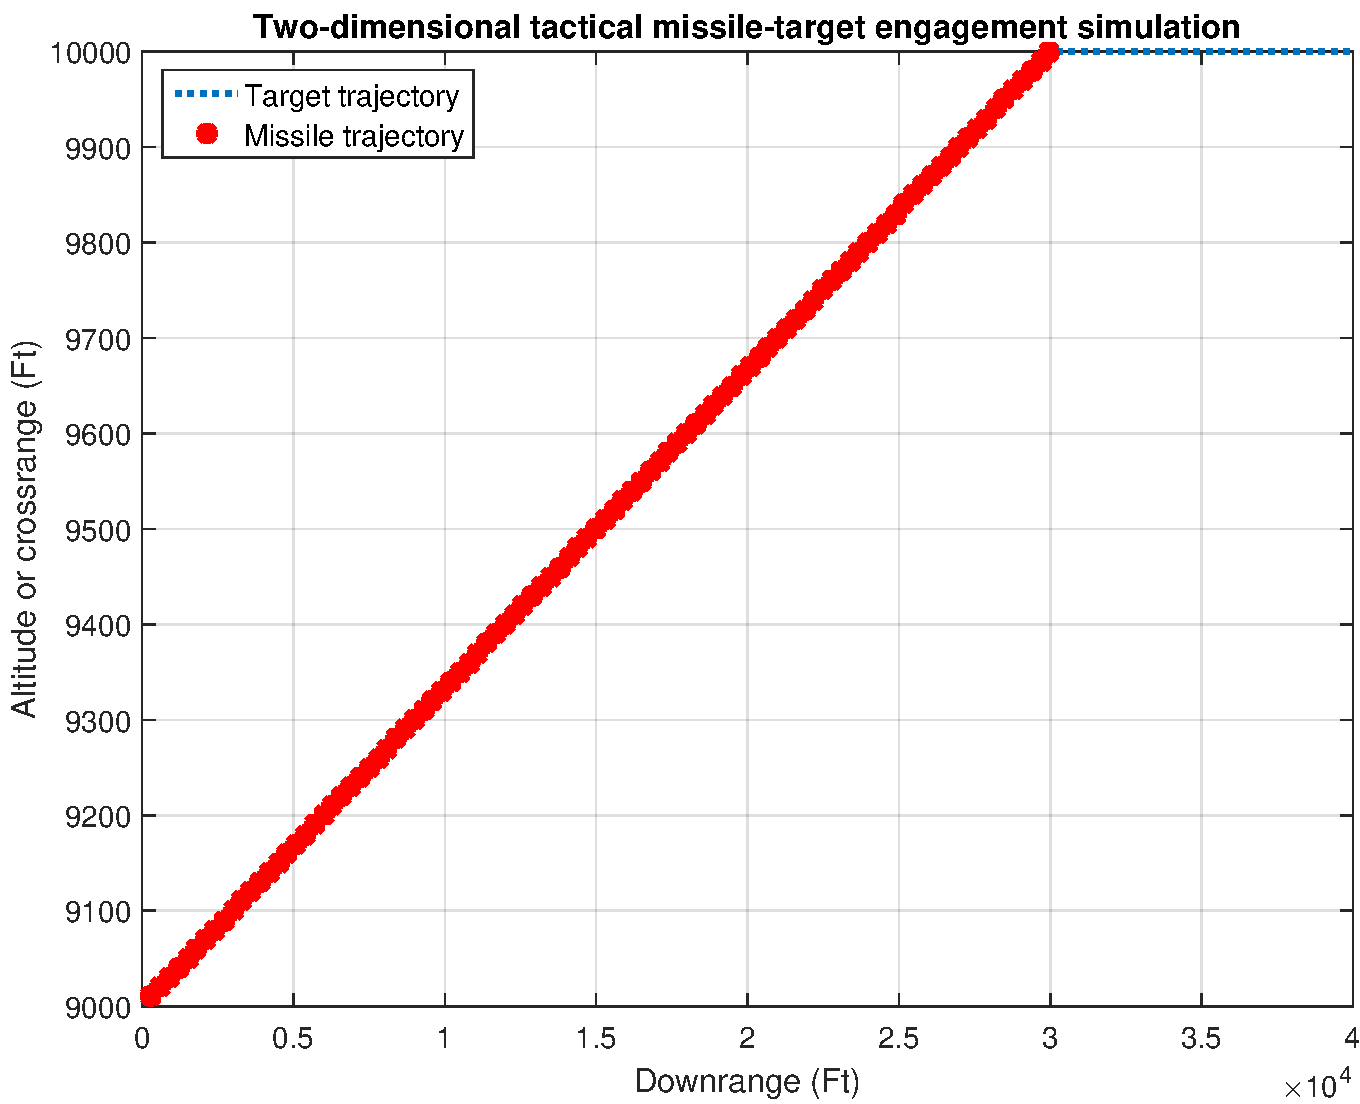
\includegraphics[scale = 0.75]{fig/trajectory0N4.pdf}
	\caption{Trajectory of the target and attacker in case of zero heading error and $N'=4$.}
	\label{trajectory0N4}
\end{figure}


\begin{figure}[htb]
	\centering
	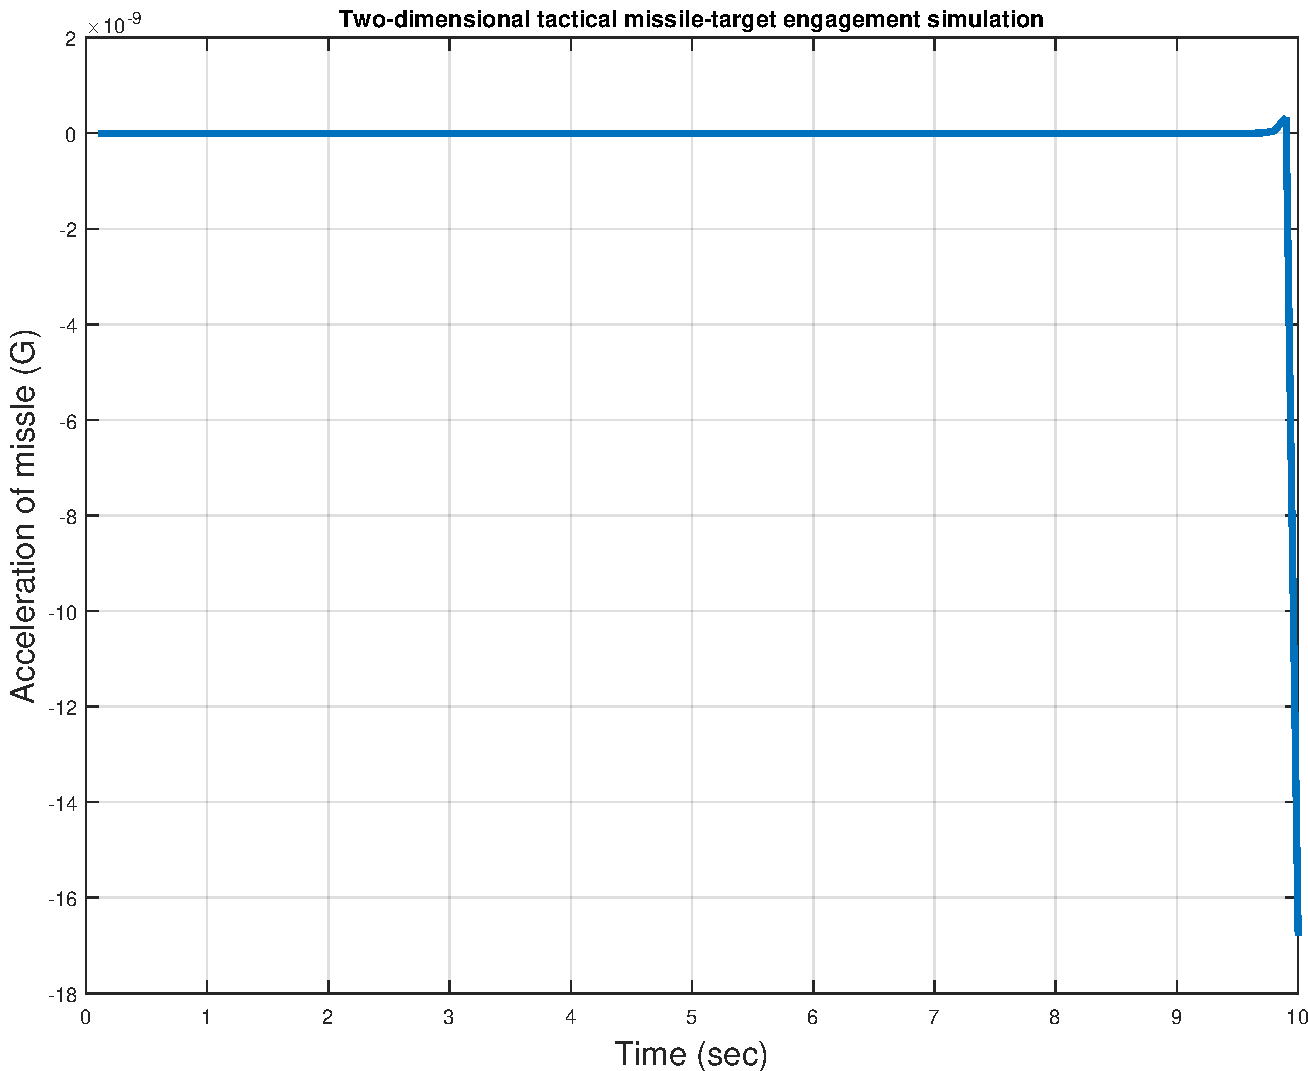
\includegraphics[scale = 0.75]{fig/MissileAcceleration0N4.pdf}
	\caption{Missile acceleration in case of zero heading error and $N'=4$ .}
	\label{missile acceleration0N4}
\end{figure}


In the case of \textbf{Heading error = -20} increasing the effective navigation ratio causes heading error to be removed rapidly as we see from  Fig. \ref{trajectory20N3}, Fig. \ref{trajectory20N4} and Fig. \ref{trajectory20N5}. The effective navigation ratio has an effect on the acceleration of the missile; the way that the missile will bleed energy as we see from Fig. \ref{missile acceleration20N3} , Fig. \ref{missile acceleration20N4} and Fig. \ref{missile acceleration20N5}. The total acceleration (area under the curve) is increasing inversely proportional with the effective navigation ratio $N'$ .


\begin{figure}[htb]
	\centering
	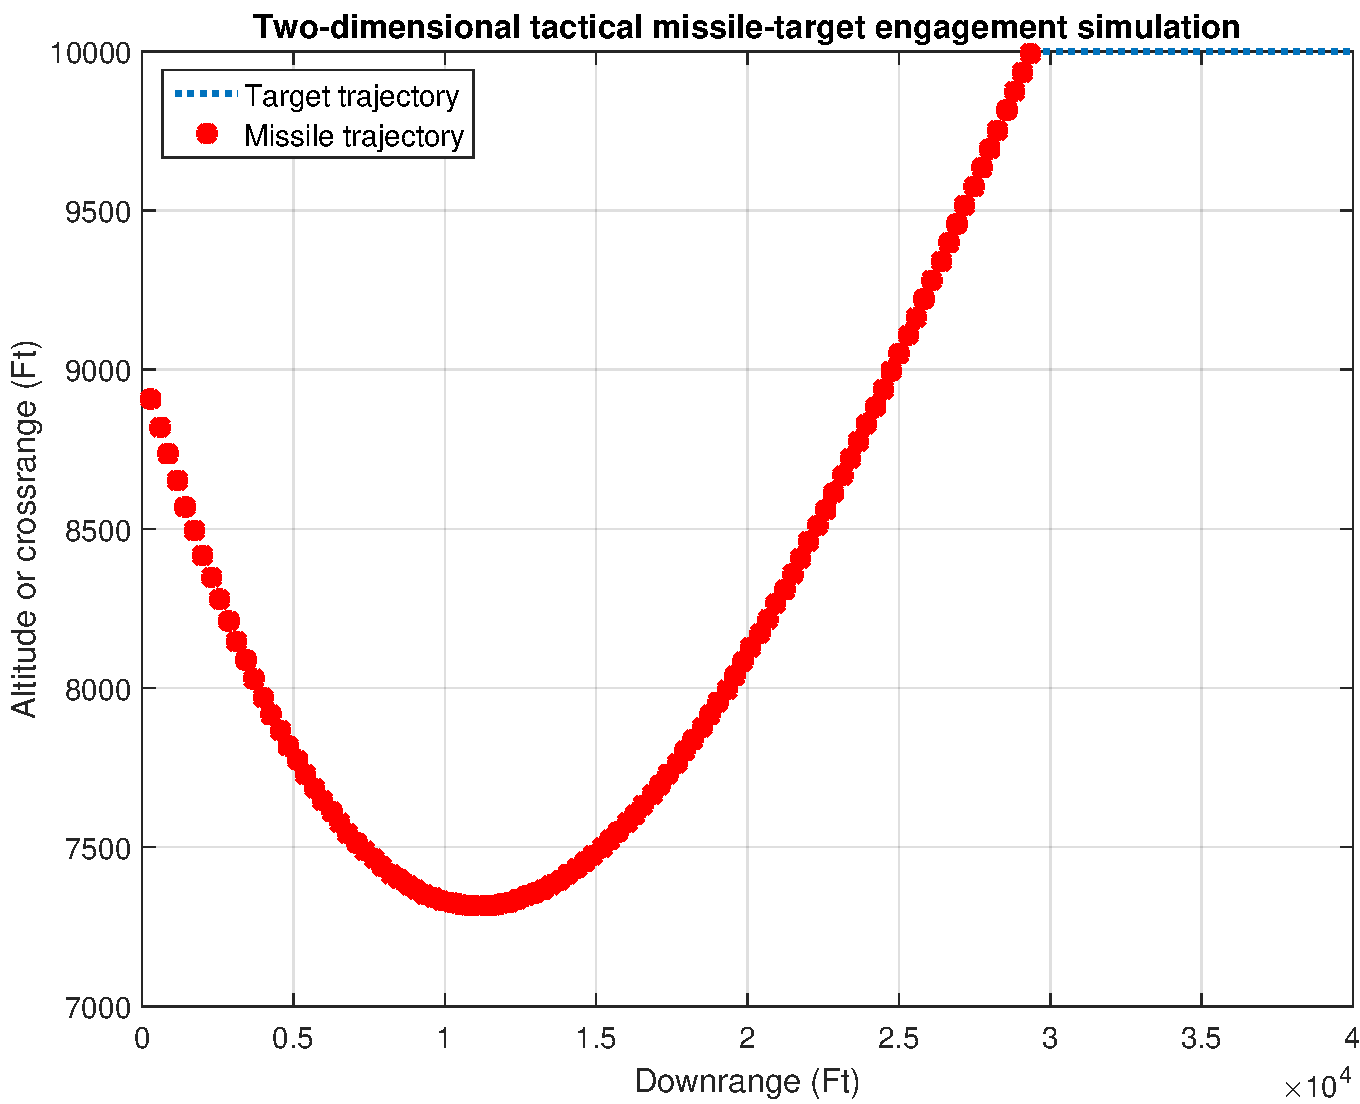
\includegraphics[scale = 0.75]{fig/trajectory20N3.pdf}
	\caption{Trajectory of the target and attacker in case of heading error=-20 and $N'=3$.}
	\label{trajectory20N3}
\end{figure}

\begin{figure}[htb]
	\centering
	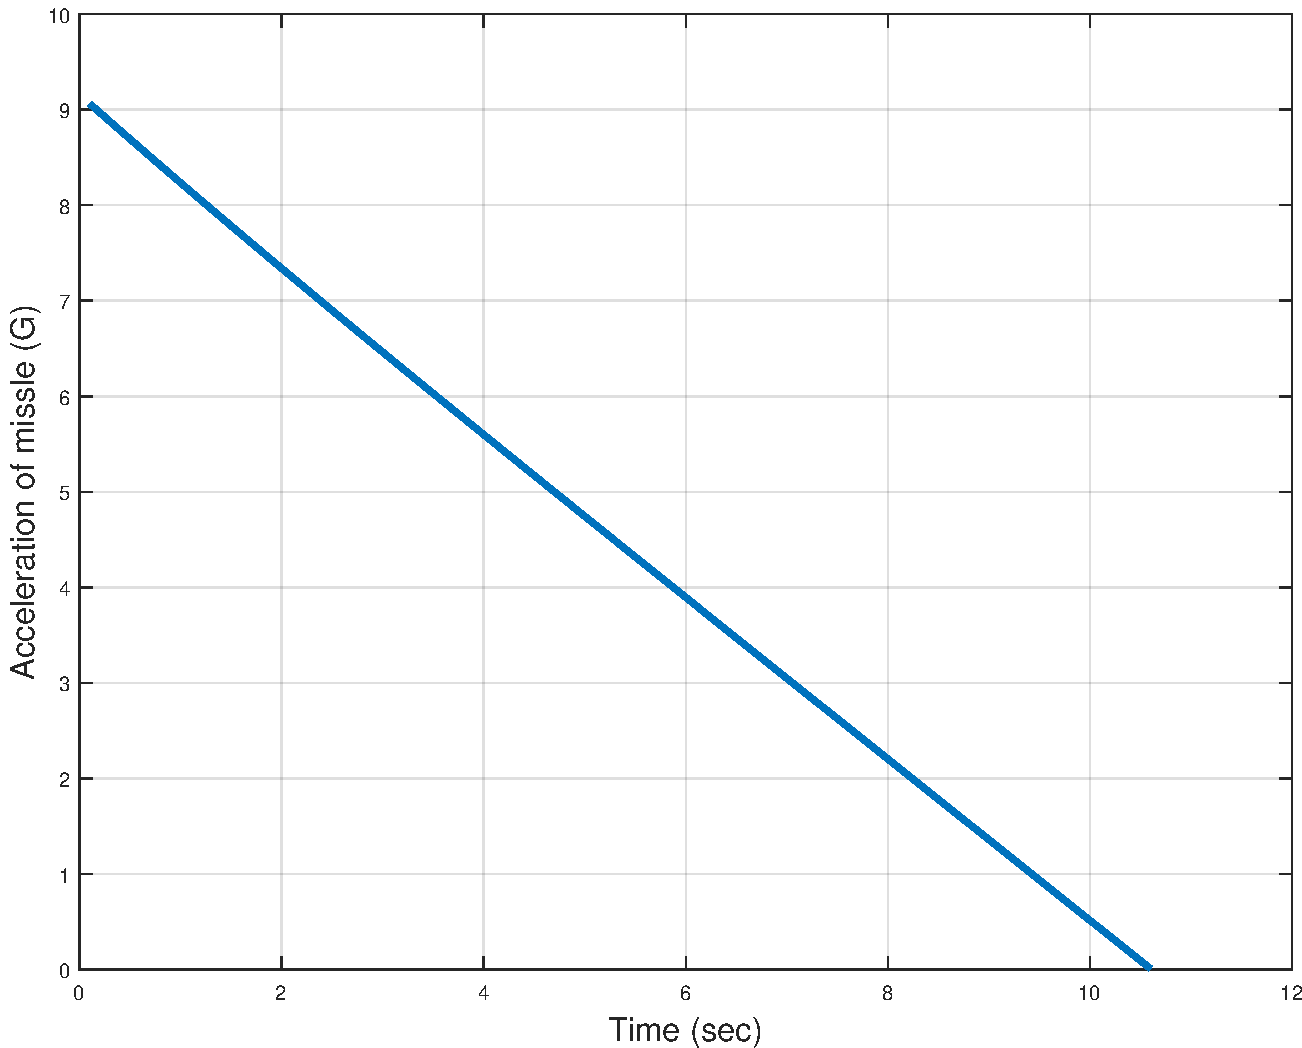
\includegraphics[scale = 0.75]{fig/MissileAcceleration20N3.pdf}
	\caption{Missile acceleration in case of heading error=-20 and $N'=3$ .}
	\label{missile acceleration20N3}
\end{figure}


\begin{figure}[htb]
	\centering
	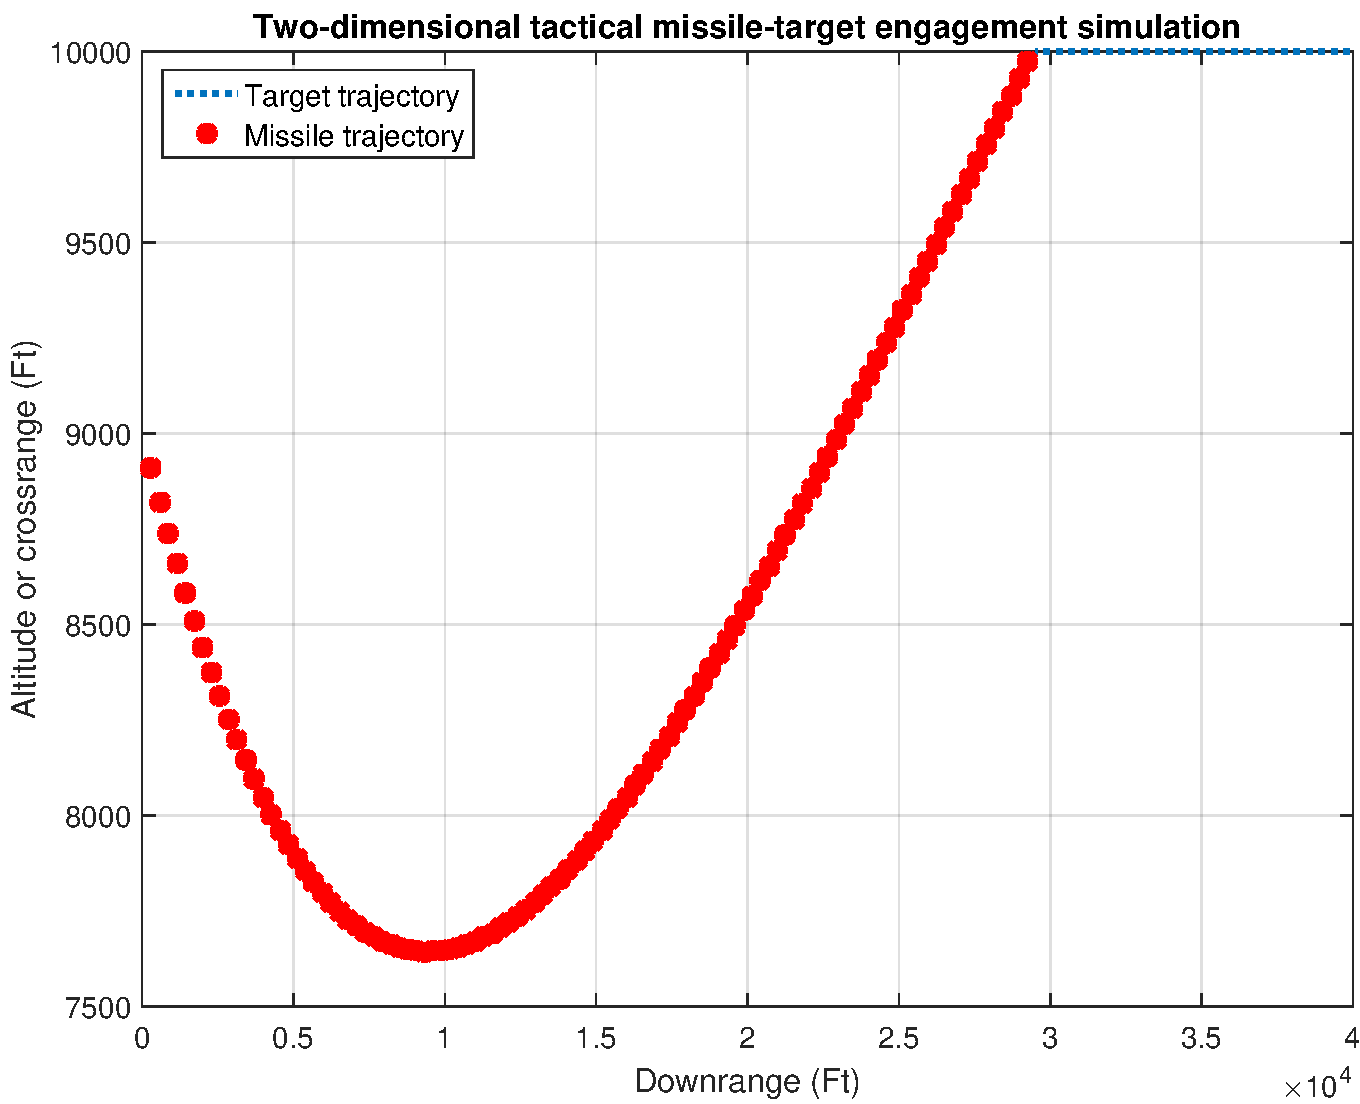
\includegraphics[scale = 0.75]{fig/trajectory20N4.pdf}
	\caption{Trajectory of the target and attacker in case of heading error=-20 and $N'=4$.}
	\label{trajectory20N4}
\end{figure}


\begin{figure}[htb]
	\centering
	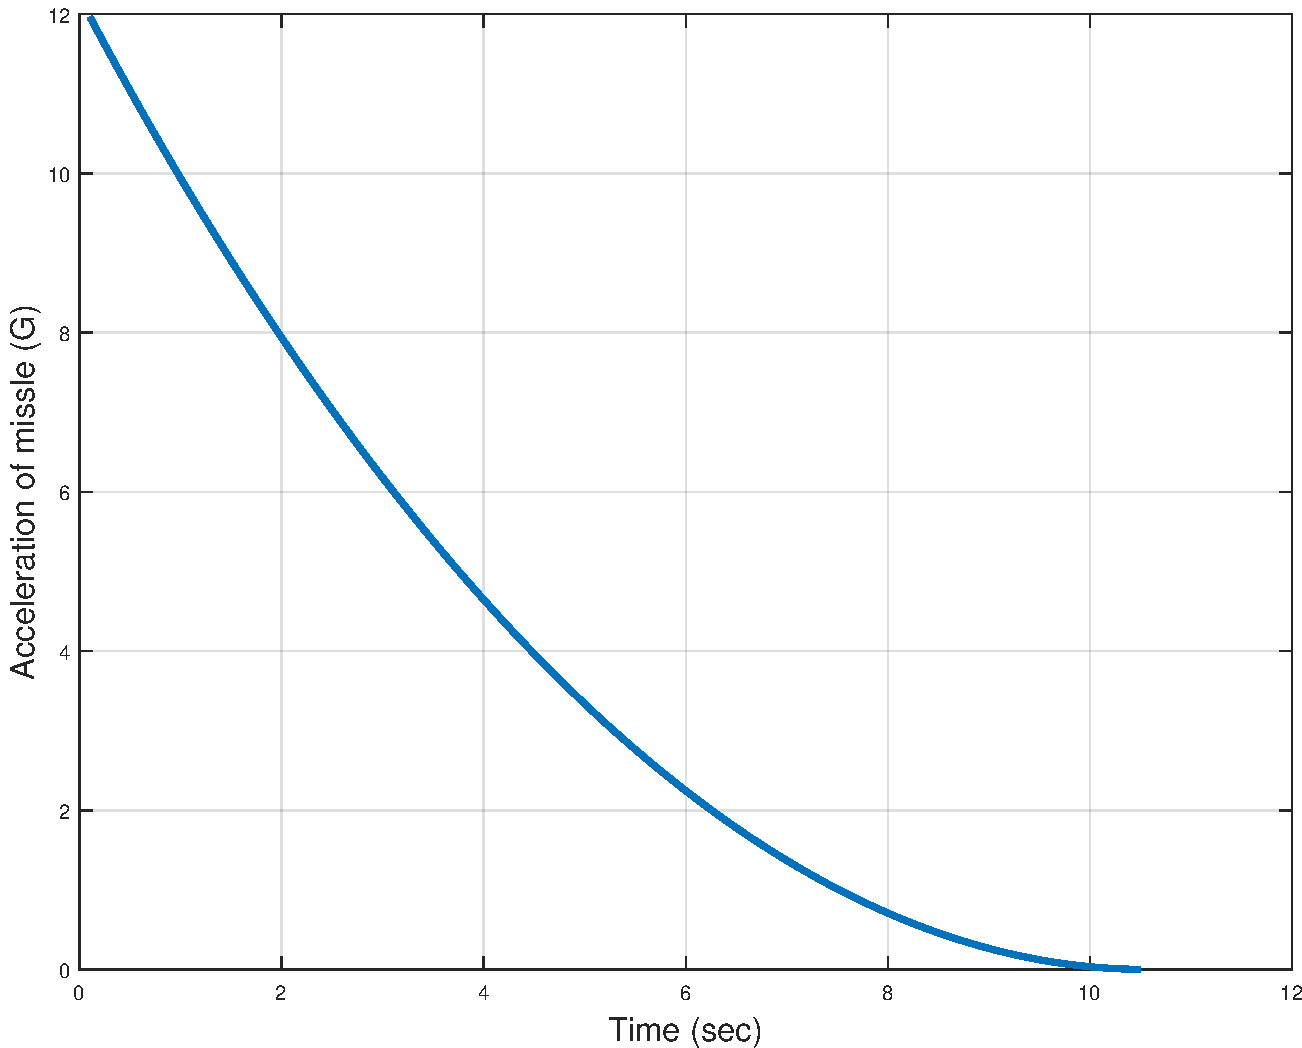
\includegraphics[scale = 0.75]{fig/MissileAcceleration20N4.pdf}
	\caption{Missile acceleration in case of heading error=-20 and $N'=4$ .}
	\label{missile acceleration20N4}
\end{figure}


\begin{figure}[htb]
	\centering
	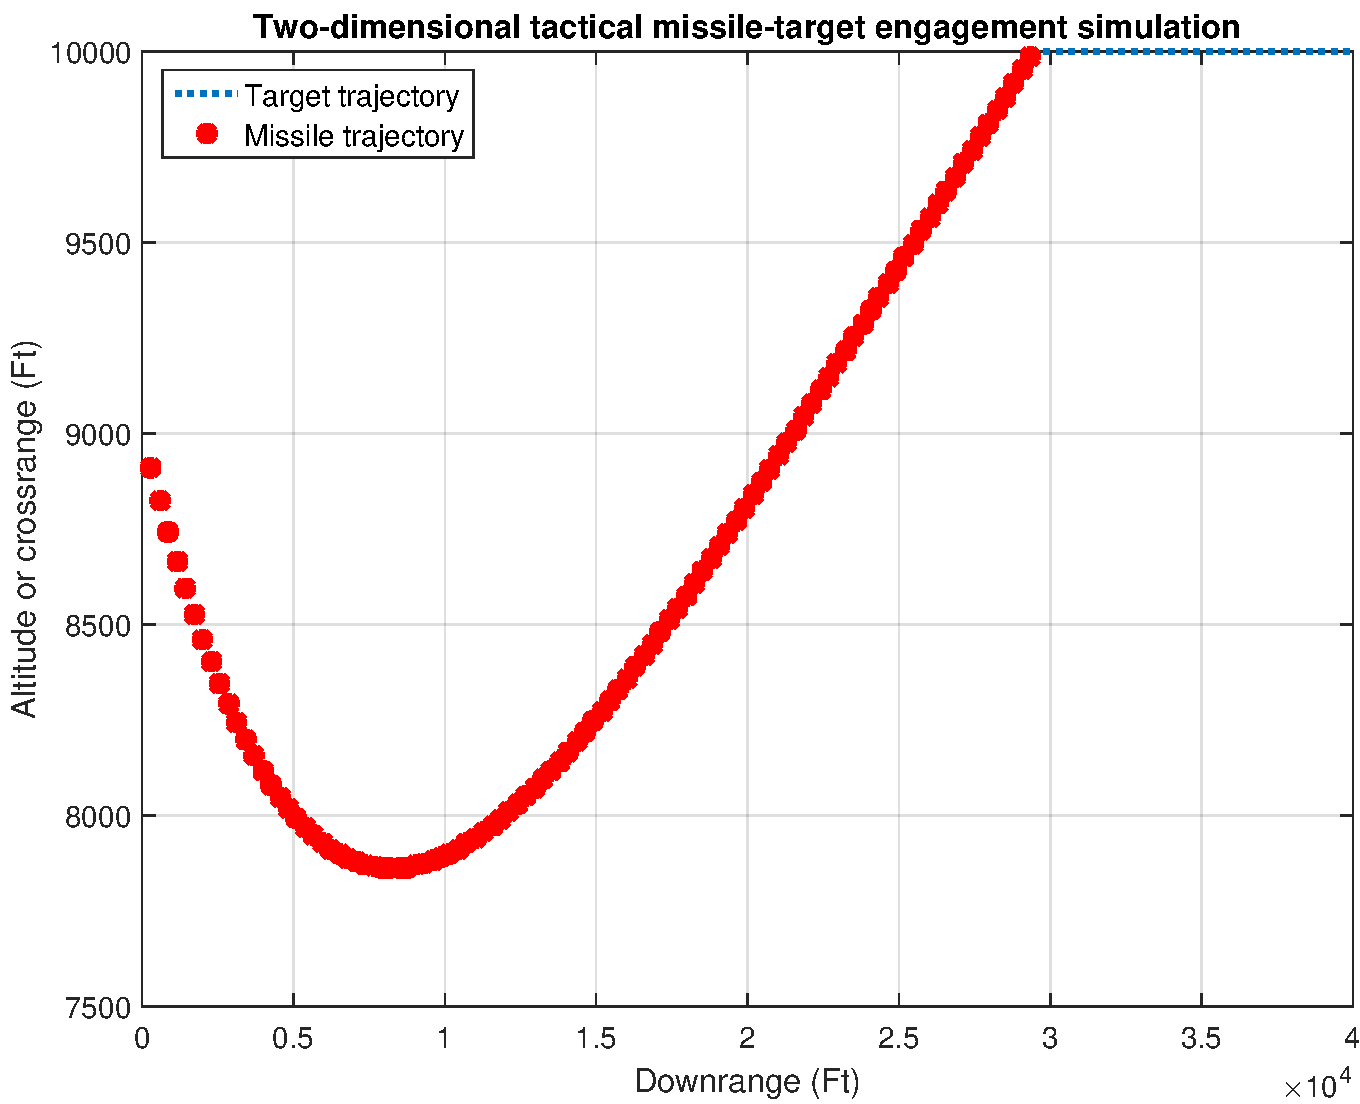
\includegraphics[scale = 0.75]{fig/trajectory20N5.pdf}
	\caption{Trajectory of the target and attacker in case of heading error=-20 and $N'=5$.}
	\label{trajectory20N5}
\end{figure}


\begin{figure}[htb]
	\centering
	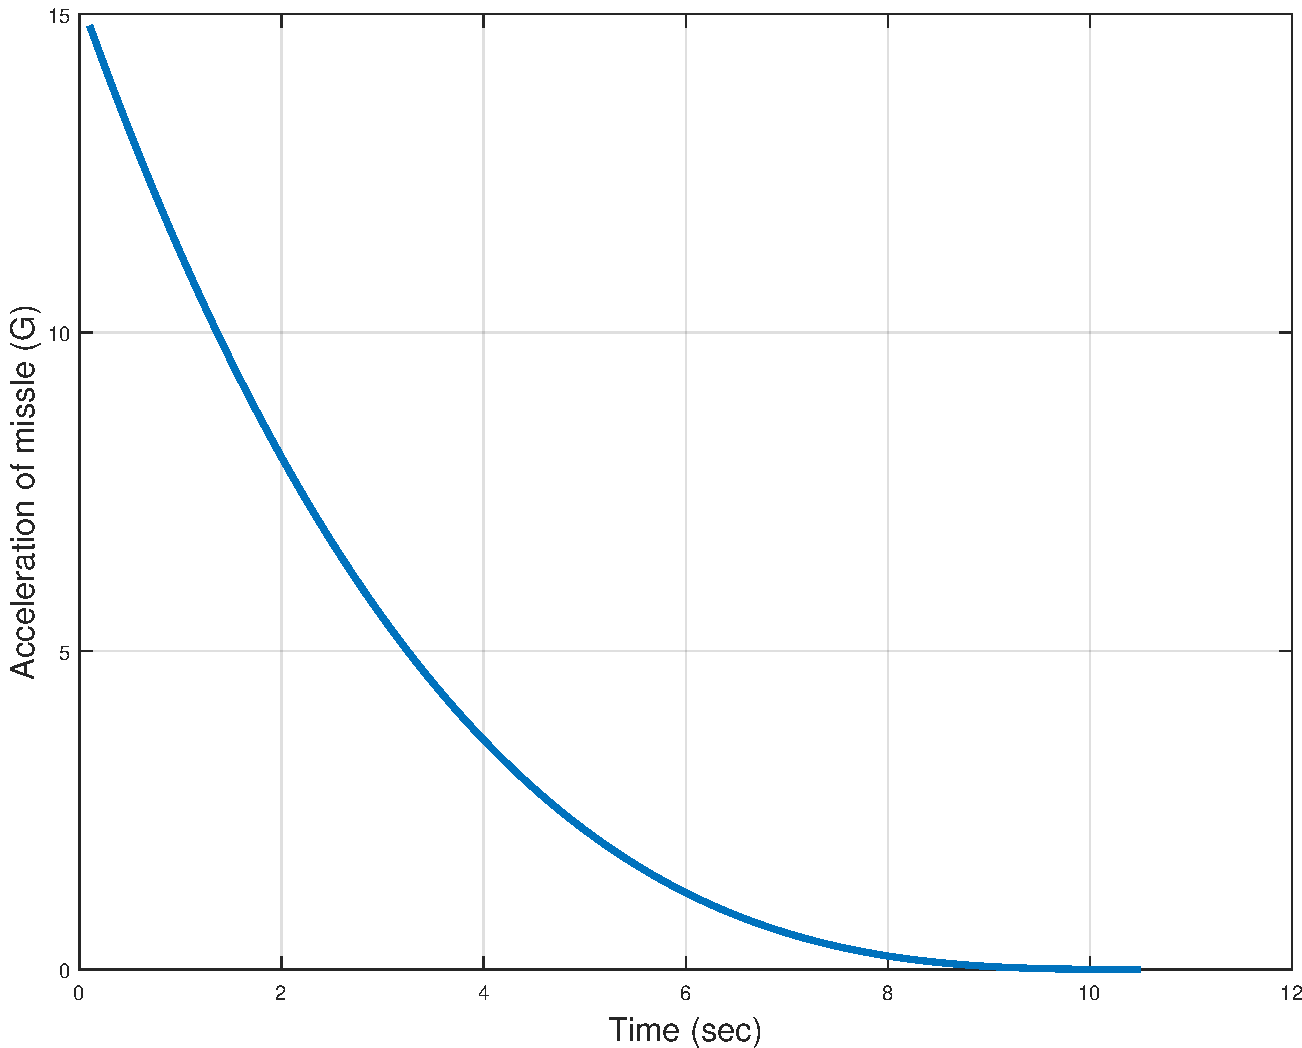
\includegraphics[scale = 0.75]{fig/MissileAcceleration20N5.pdf}
	\caption{Missile acceleration in case of heading error=-20 and $N'=5$ .}
	\label{missile acceleration20N5}
\end{figure}

%-----------------------------------------------------------

\subsubsection{Constant Target maneuver}
In this case the target does some effort to escape from the attacker, in the form of constant acceleration (in our example target acceleration = $3g=96.6$).
We see from Fig. \ref{missile acceleration0NN3} and Fig. \ref{missile acceleration0NN5} that a higher effective navigation ratio yields less acceleration to hit maneuvering target, and causes the missile to lead the target slightly more than a lower effective navigation ratio does, as we see from Fig. \ref{trajectory0NN3} and Fig. \ref{trajectory0NN3}.



\begin{figure}[htb]
	\centering
	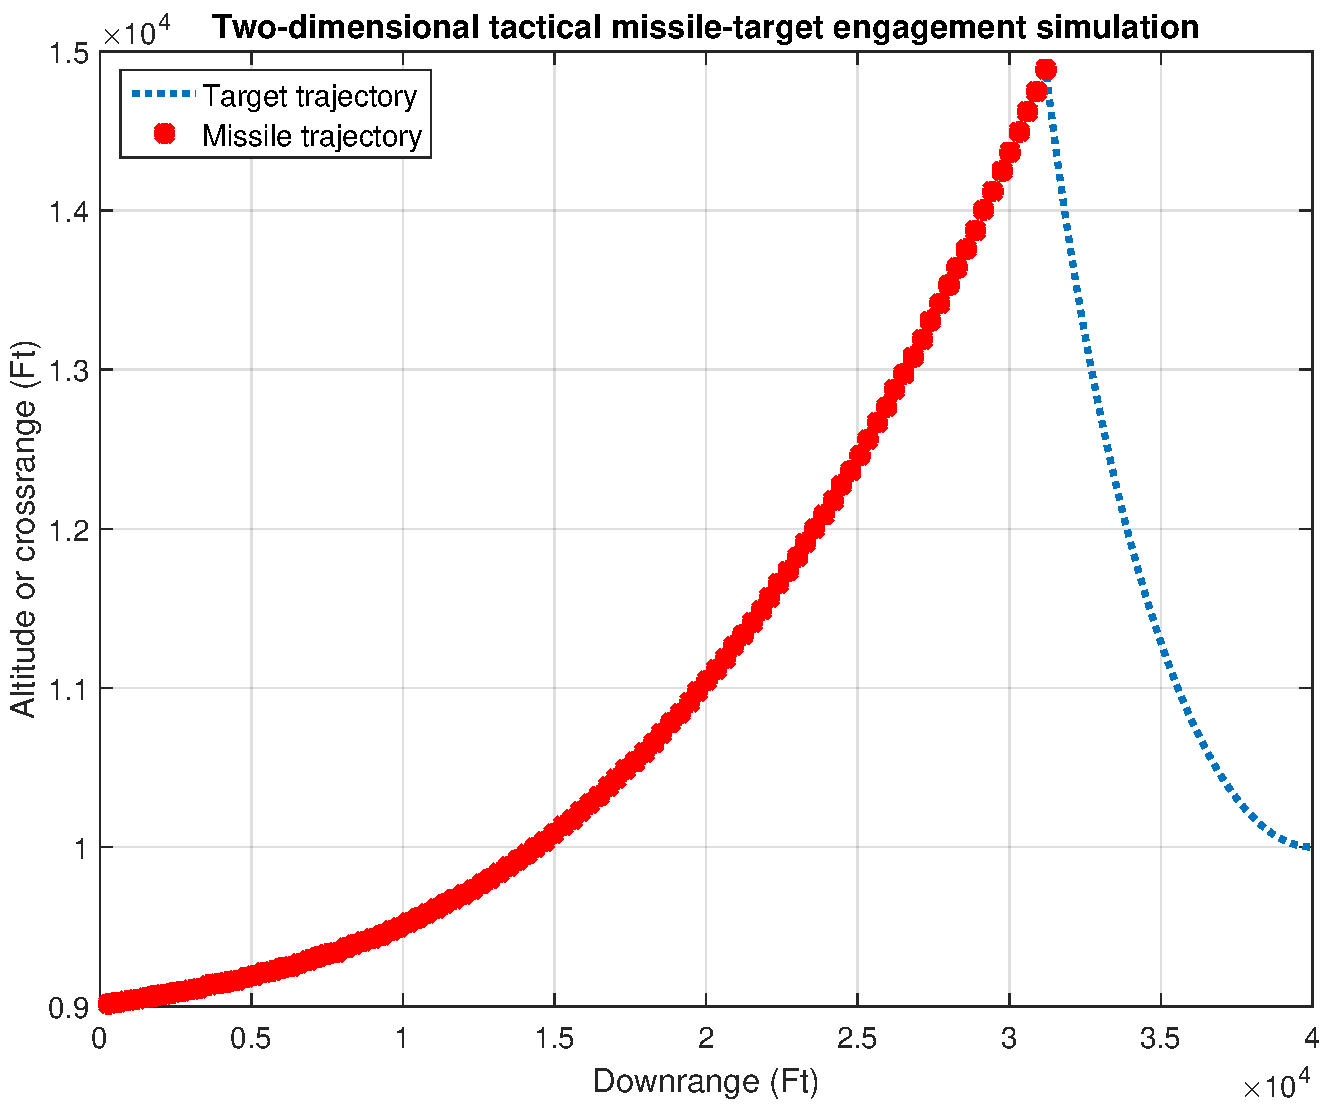
\includegraphics[scale = 0.75]{fig/trajectory0NN3.pdf}
	\caption{Trajectory of the target and attacker in case of heading error=0 and $N'=3$.}
	\label{trajectory0NN3}
\end{figure}


\begin{figure}[htb]
	\centering
	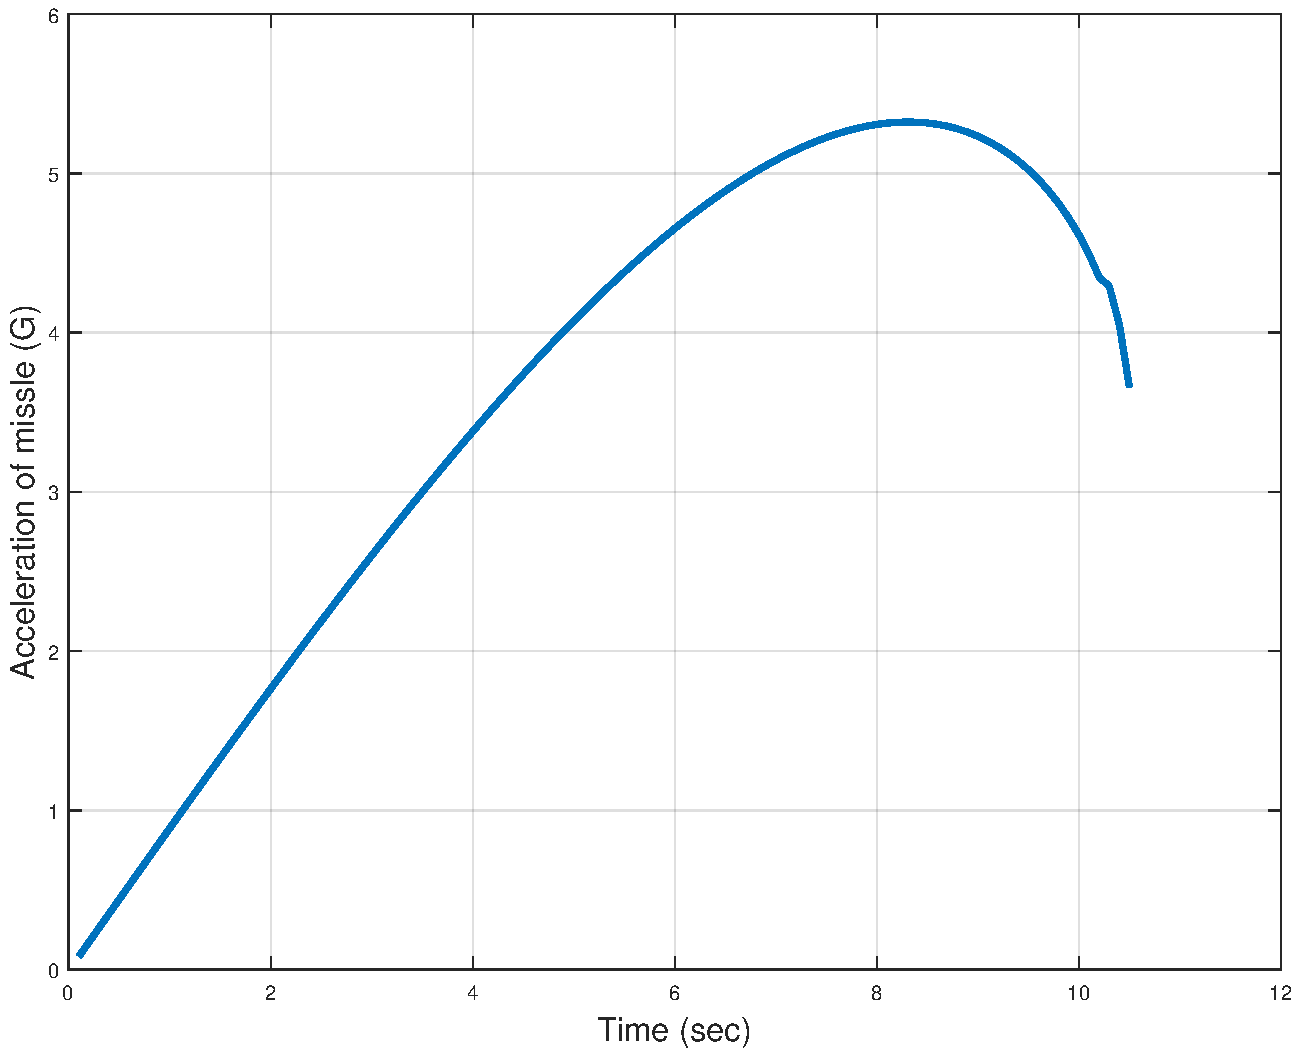
\includegraphics[scale = 0.75]{fig/MissileAcceleration0NN3.pdf}
	\caption{Missile acceleration in case of heading error=0 and $N'=3$ .}
	\label{missile acceleration0NN3}
\end{figure}



\begin{figure}[htb]
	\centering
	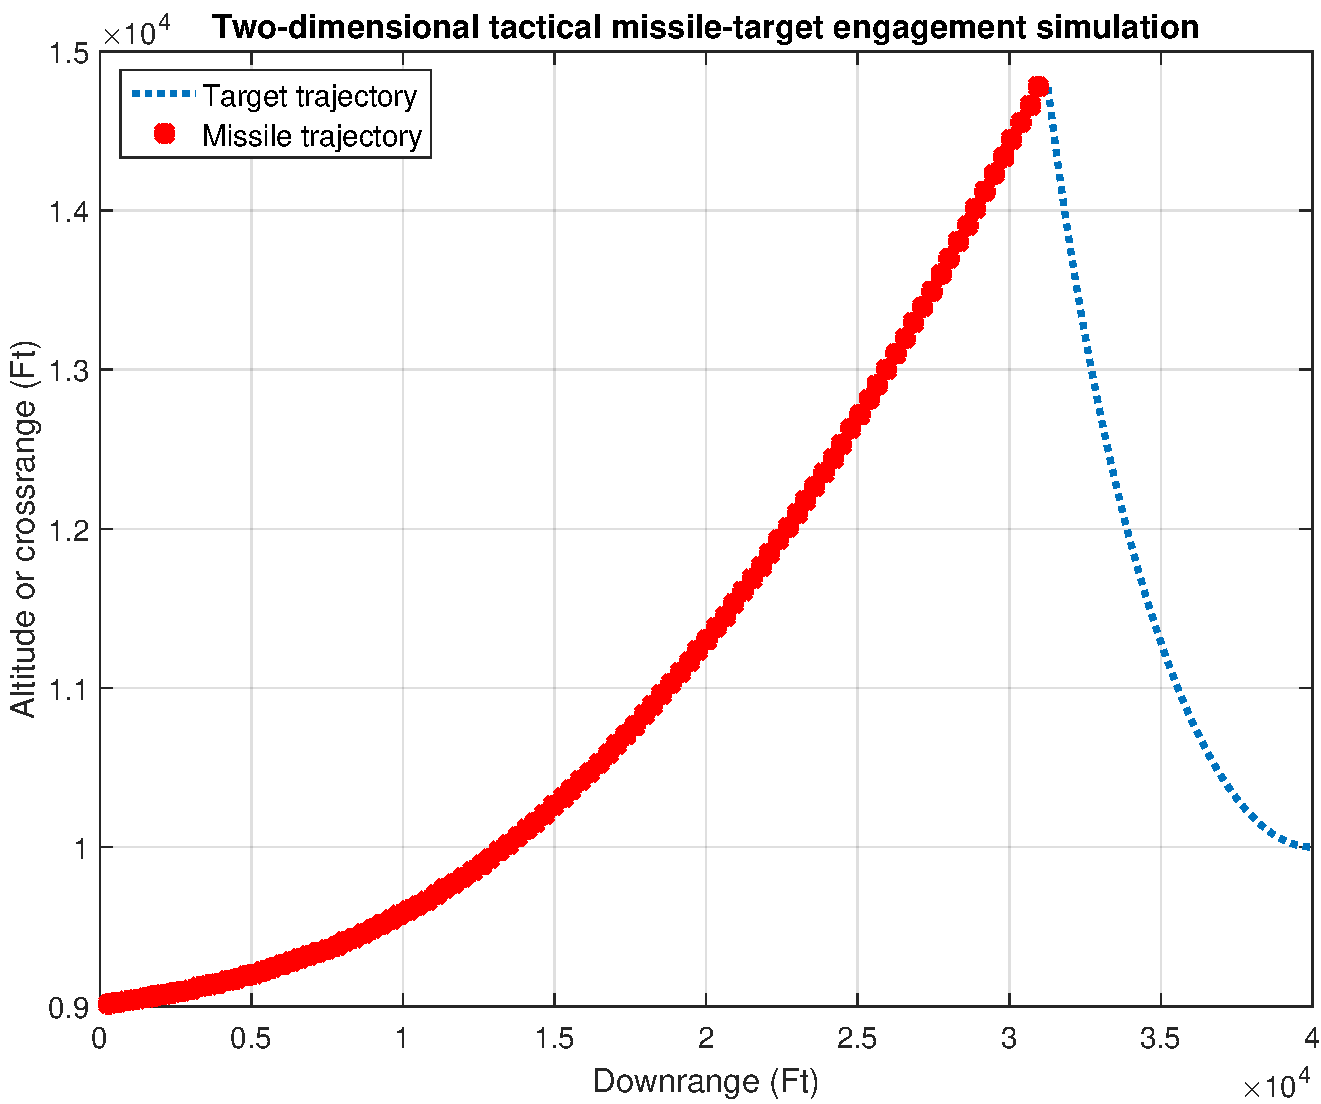
\includegraphics[scale = 0.75]{fig/trajectory0NN5.pdf}
	\caption{Trajectory of the target and attacker in case of heading error=0 and $N'=5$.}
	\label{trajectory0NN5}
\end{figure}


\begin{figure}[htb]
	\centering
	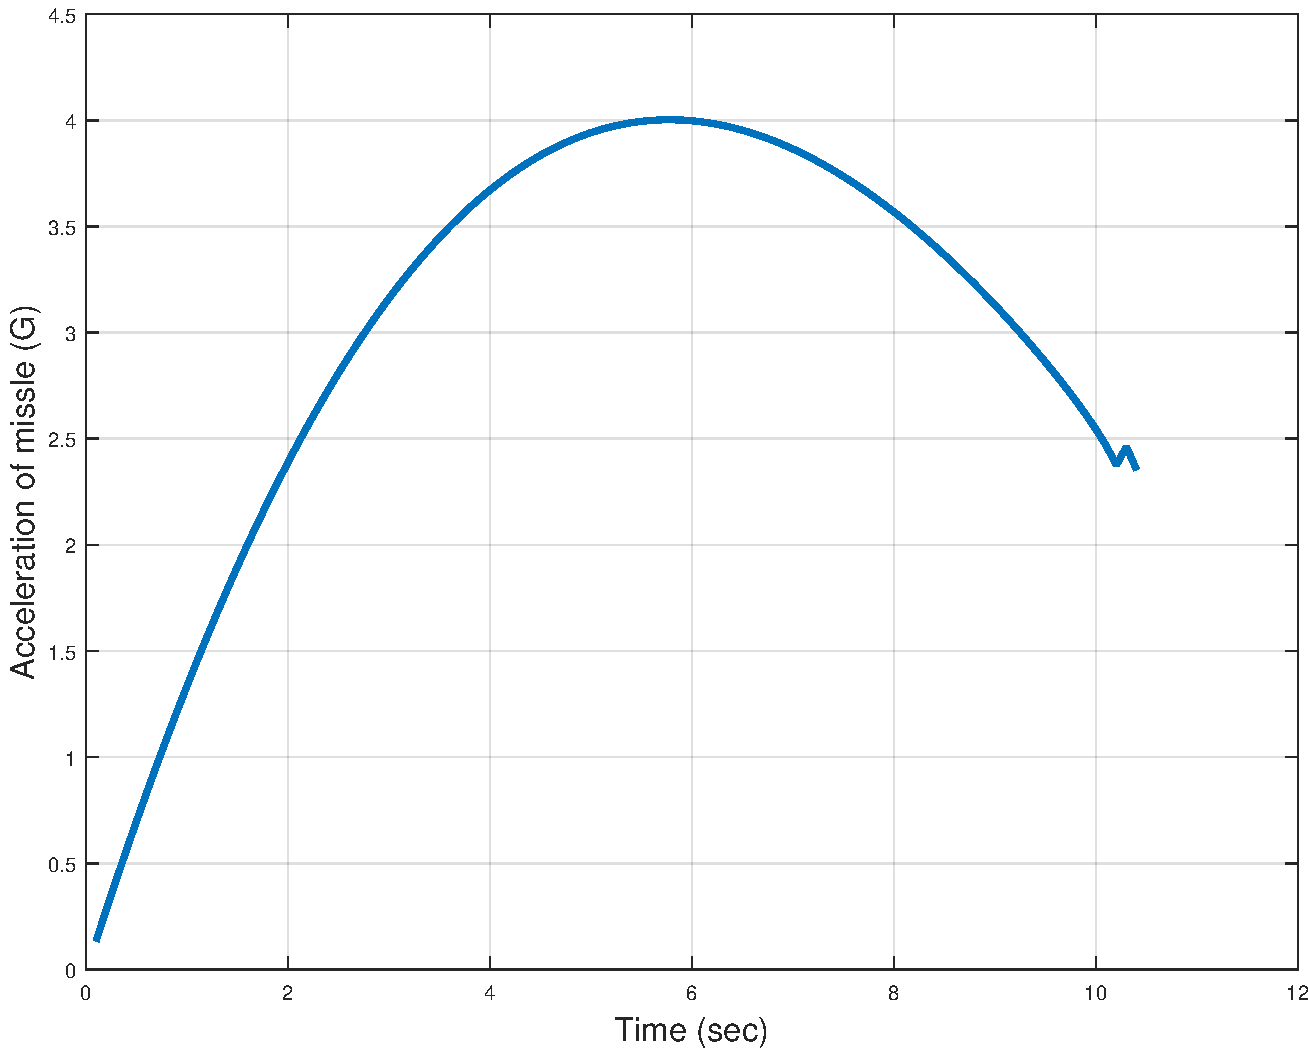
\includegraphics[scale = 0.75]{fig/MissileAcceleration0NN5.pdf}
	\caption{Missile acceleration in case of heading error=0 and $N'=5$ .}
	\label{missile acceleration0NN5}
\end{figure}
%-----------------------------------------------------------

\subsubsection{Polynomial Target maneuver}
Now we will make the Target maneuver as a polynomial in the form

\begin{equation}
	f(t) = c_0 + c_1 T + c_2 T^2 + c_3 T^3 + ... + c_N T^N
\end{equation} 

where T is time , c are unknown coefficients of the polynomial and N is the polynomial degree.
In our simulation we choose N reasonably $3\to5$ and the coefficients are randomly generated then we solve the proportional navigation equations to get values for two important parameters, namely the miss distance and the command acceleration for the Missile. Then, we calculate the cost function depends on these two parameters, as our target is to maximize miss distance to make the target safe, and maximize command acceleration for the missile, so it bleeds energy before it catches the target. We will do this process many times till the number of runs we need. The next figures shows the trajectories of the Target and Missile for N=3,4,5 and corresponding missile acceleration for each case.

\begin{figure}[htb]
	\centering
	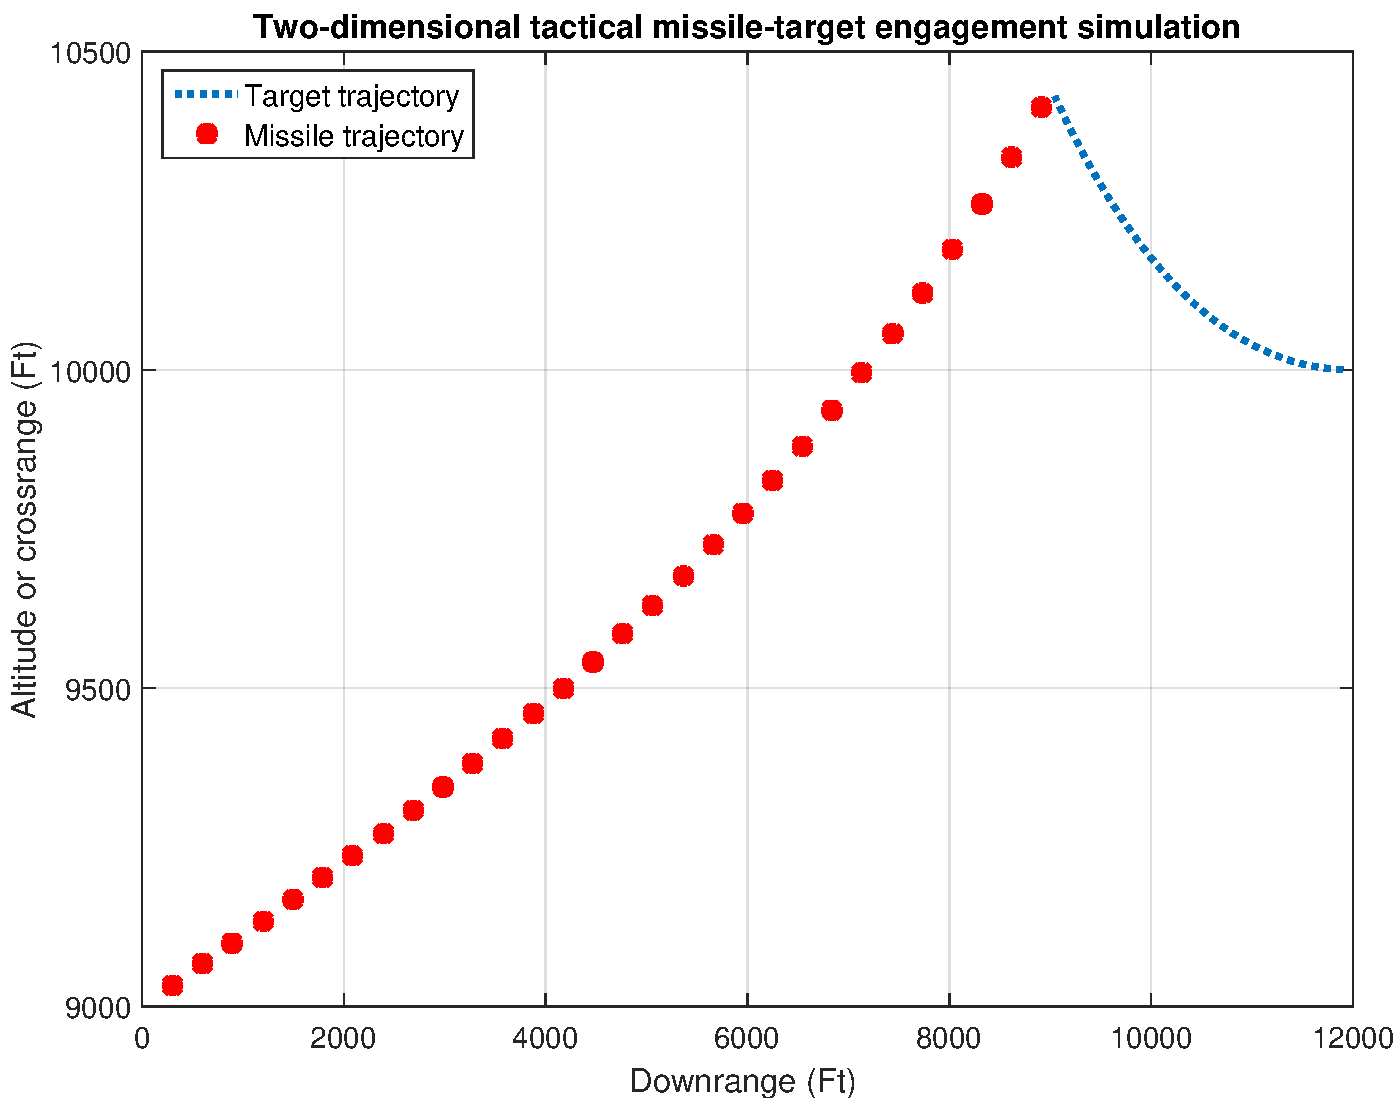
\includegraphics[scale = 0.75]{fig/trajectoryP3.pdf}
	\caption{Trajectory of the target and attacker in case of polynomial degree N=3.}
	\label{trajectoryP3}
\end{figure}


\begin{figure}[htb]
	\centering
	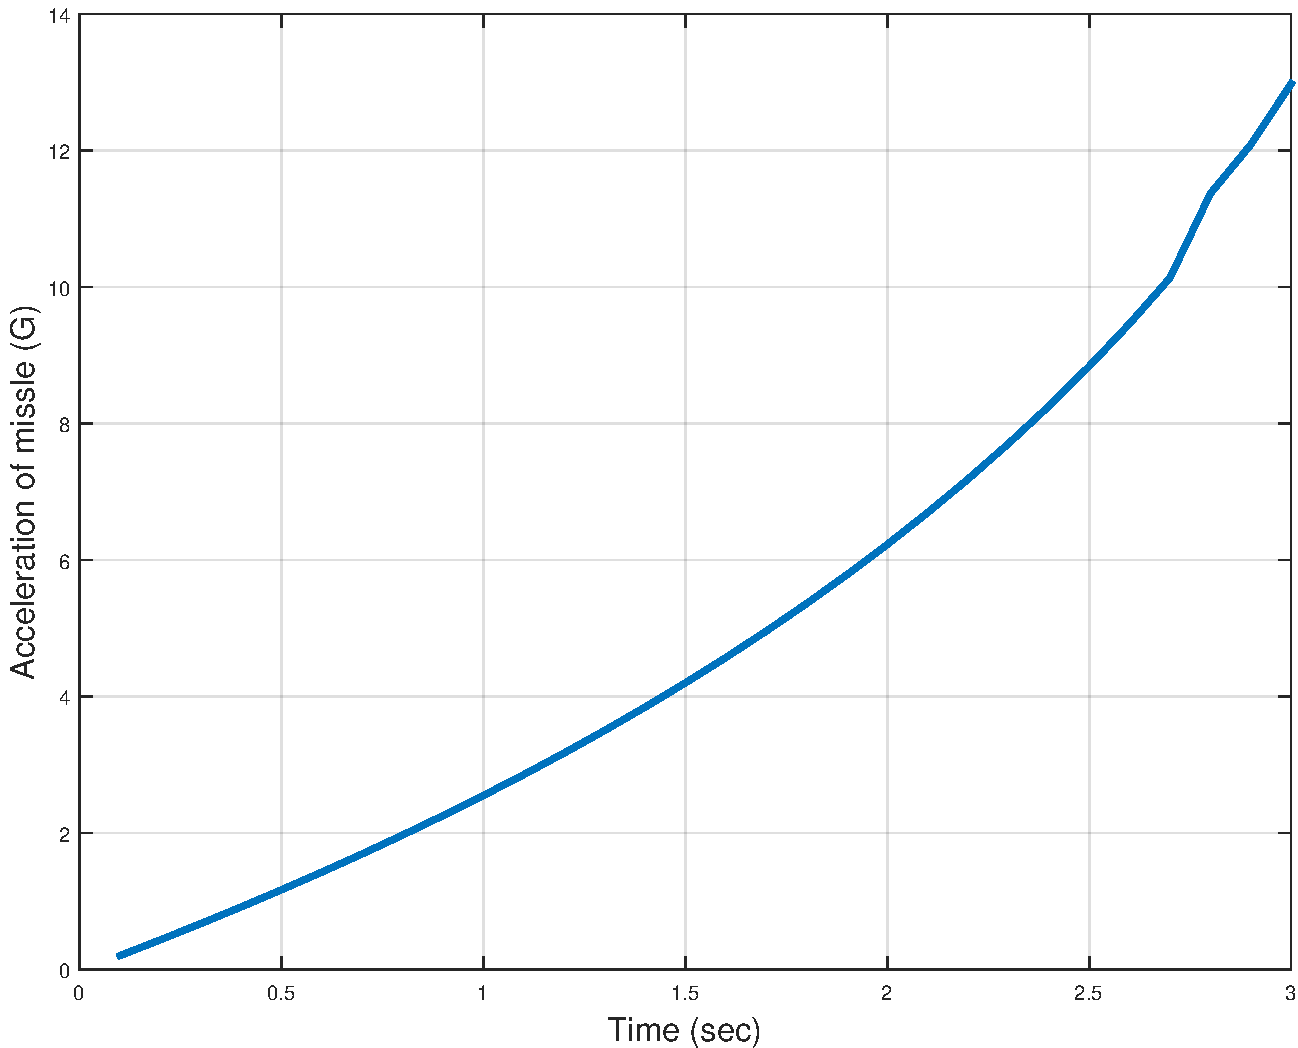
\includegraphics[scale = 0.75]{fig/MissileAccelerationP3.pdf}
	\caption{Missile acceleration in case of polynomial degree N=3.}
	\label{missile accelerationP3}
\end{figure}


\begin{figure}[htb]
	\centering
	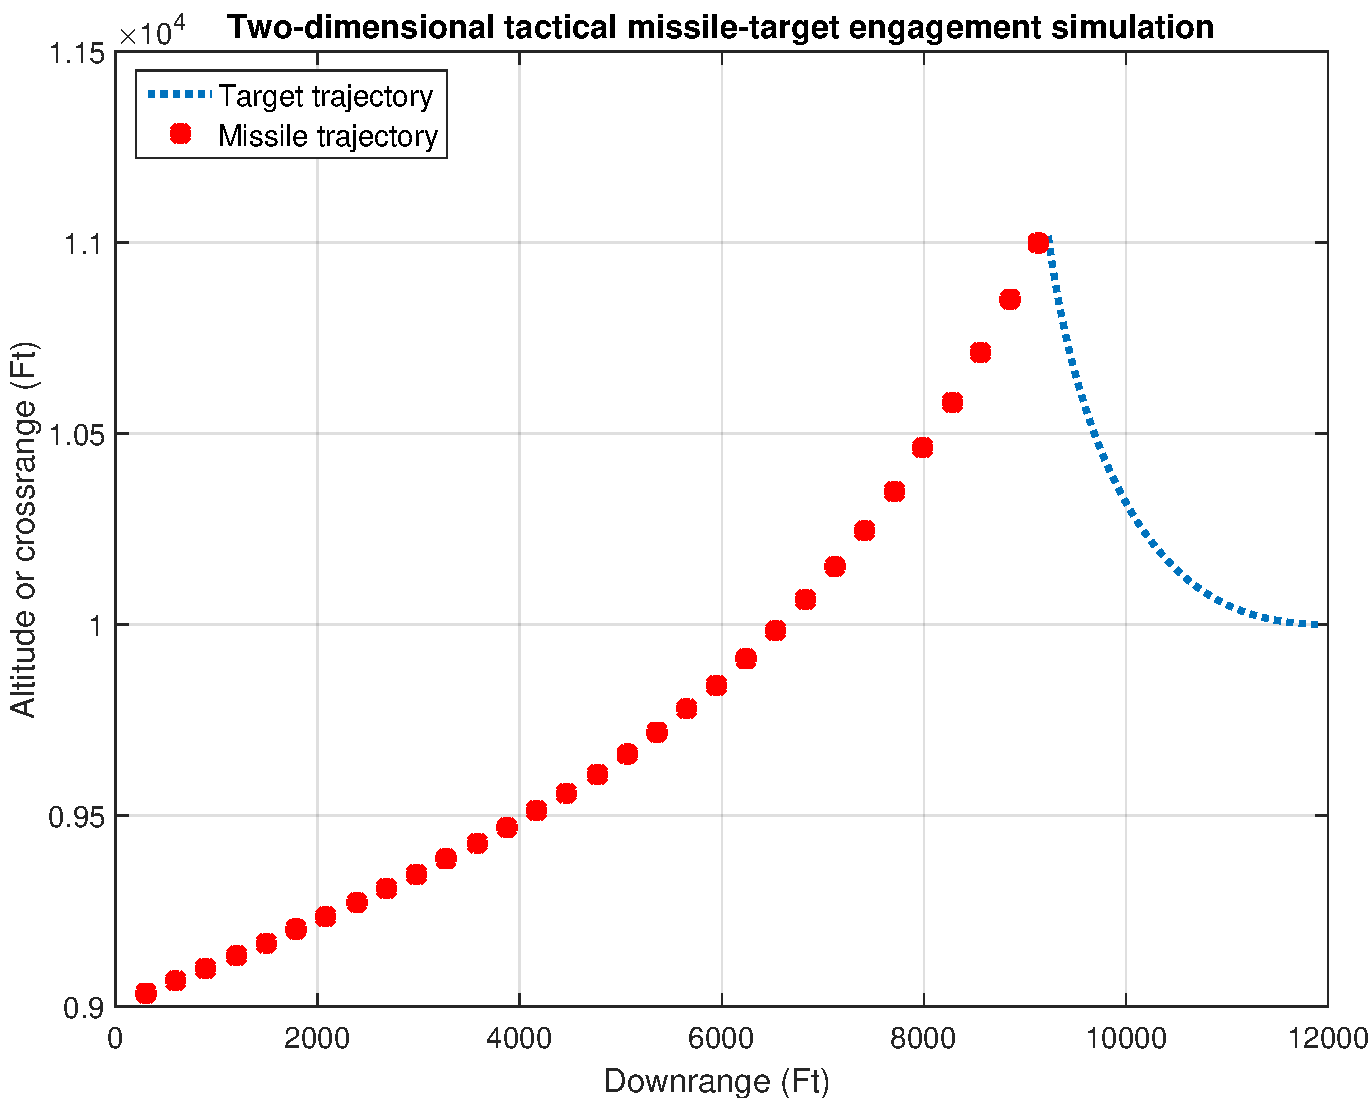
\includegraphics[scale = 0.75]{fig/trajectoryP4.pdf}
	\caption{Trajectory of the target and attacker in case of polynomial degree N=4.}
	\label{trajectoryP4}
\end{figure}


\begin{figure}[htb]
	\centering
	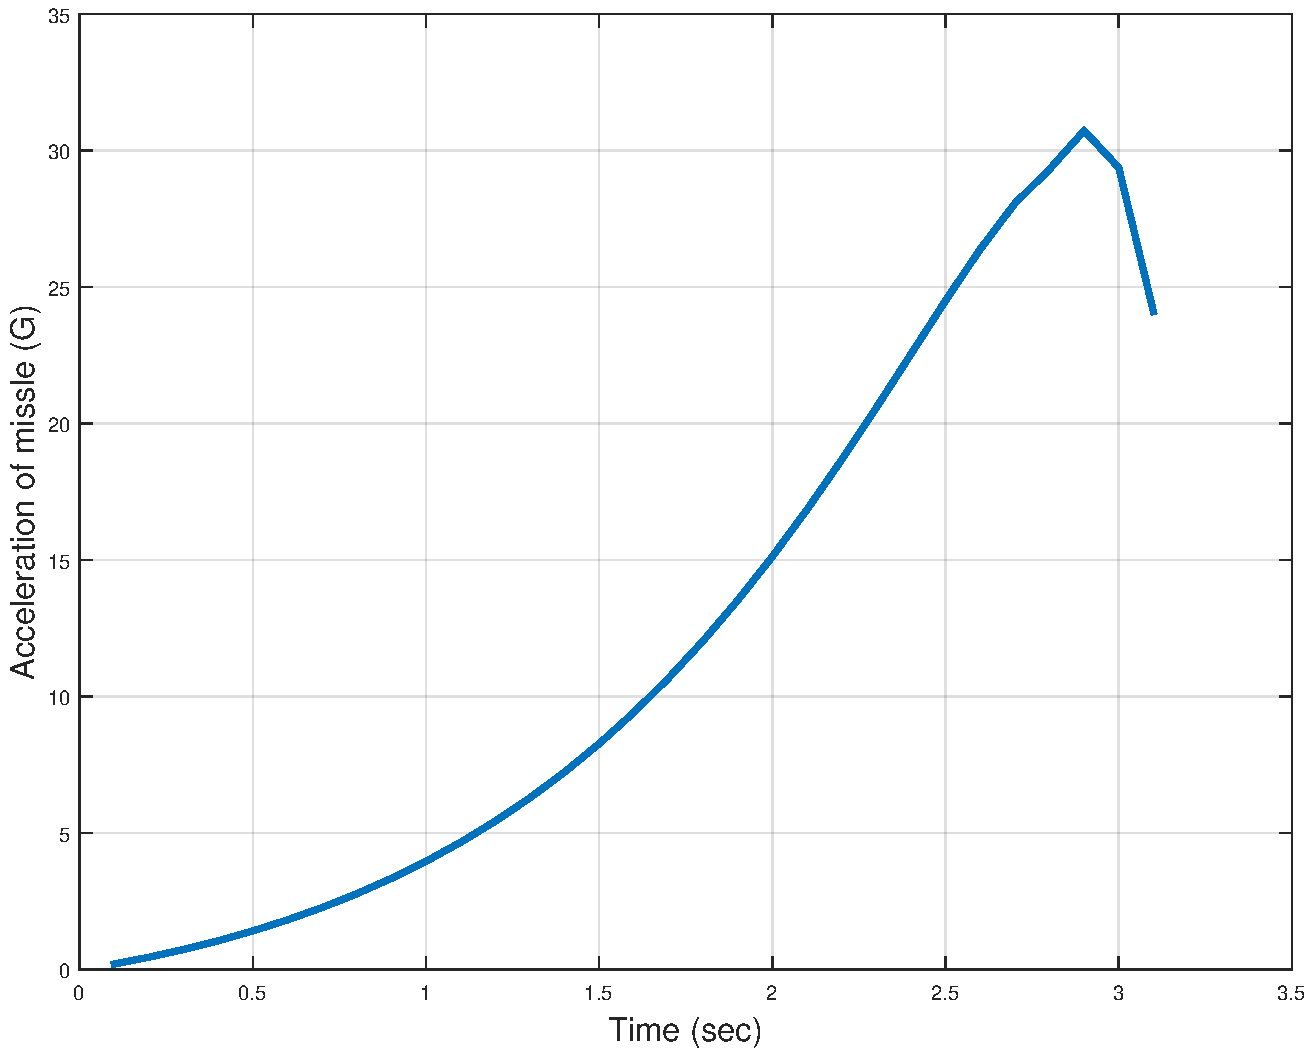
\includegraphics[scale = 0.75]{fig/MissileAccelerationP4.pdf}
	\caption{Missile acceleration in case of polynomial degree N=4.}
	\label{missile accelerationP4}
\end{figure}


\begin{figure}[htb]
	\centering
	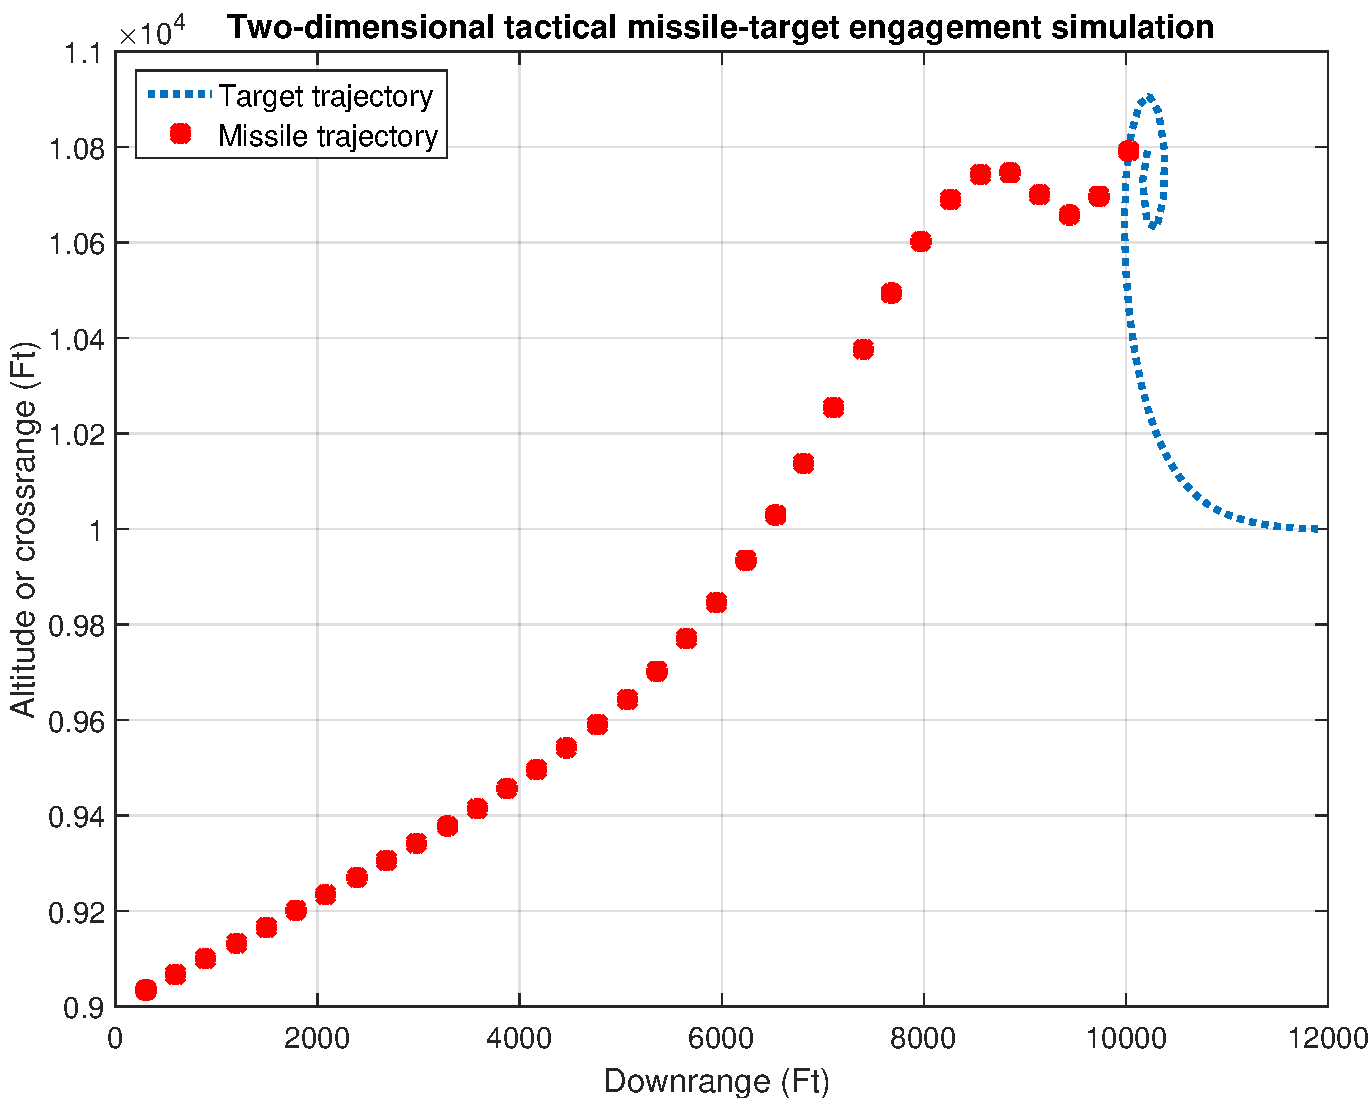
\includegraphics[scale = 0.75]{fig/trajectoryP5.pdf}
	\caption{Trajectory of the target and attacker in case of polynomial degree N=5.}
	\label{trajectoryP5}
\end{figure}


\begin{figure}[htb]
	\centering
	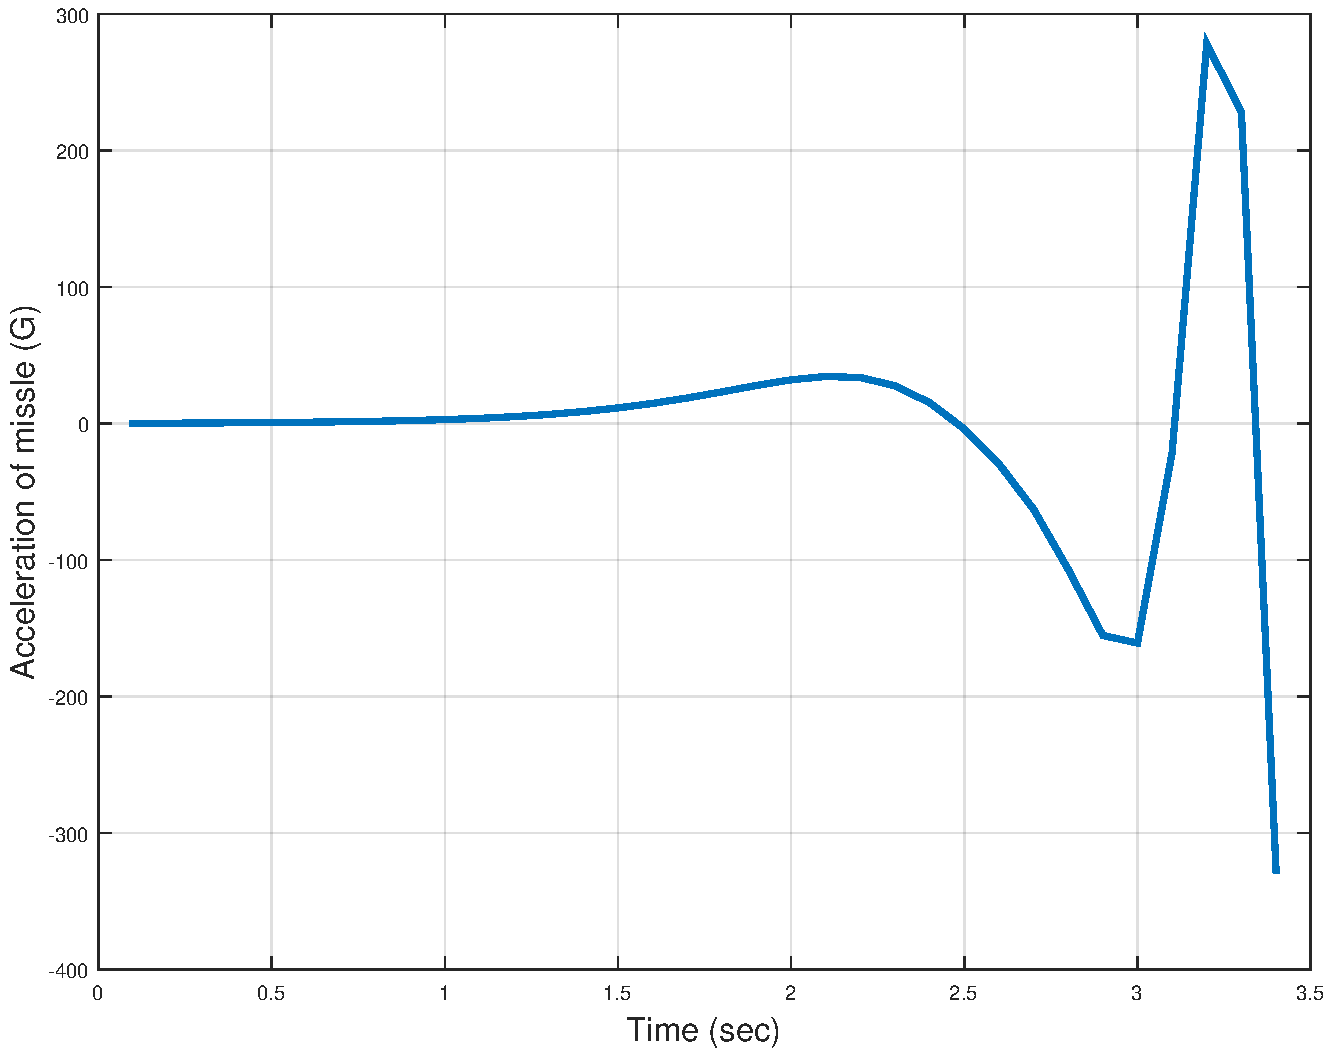
\includegraphics[scale = 0.75]{fig/MissileAccelerationP5.pdf}
	\caption{Missile acceleration in case of polynomial degree N=5.}
	\label{missile accelerationP5}
\end{figure}

%------------------------------------------------------------

\subsubsection{Trapezoidal Target maneuver}
Now we will make the Target maneuver as a trapezoidal function illustrated in Fig. \ref{trapezoidalacc}


\begin{figure}[htb]
	\centering
	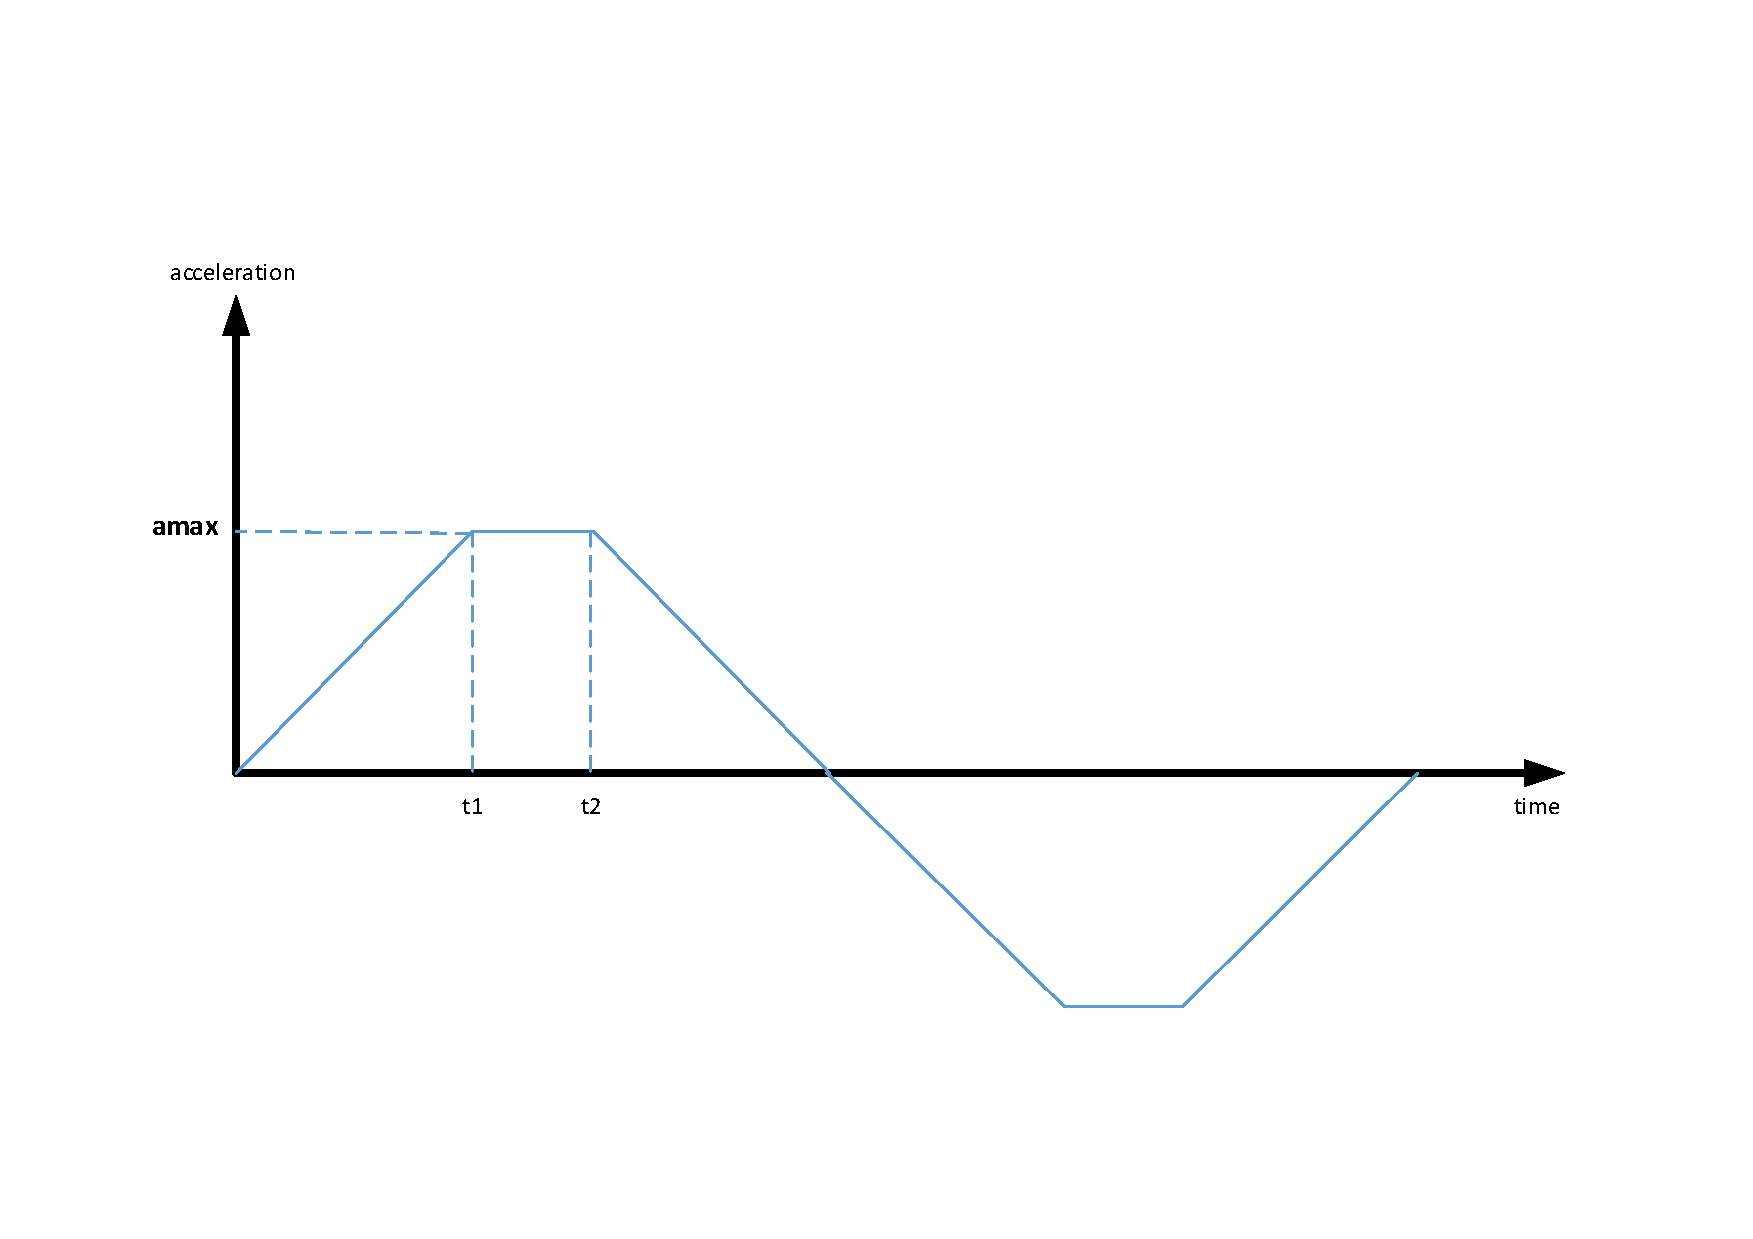
\includegraphics[scale = 0.75]{fig/trapezoidalacc.pdf}
	\caption{Trapezoidal Target maneuver.}
	\label{trapezoidalacc}
\end{figure}
In the simulation we choose the value for maximum acceleration. The time of beginning the ramp (which is 0), and the time at the end of the descent, $t_1$ and $t_2$ are randomly generated. Then we calculate the cost function which depends on the values of the miss distance and Missile acceleration and we do this process several runs till we find $t_1$ and $t_2$ that maximize miss distance and missile acceleration.   
The advantage of this form is that we can control the values of maximum acceleration to adapt with the acceleration the pilot can withstand.

\begin{figure}[htb]
	\centering
	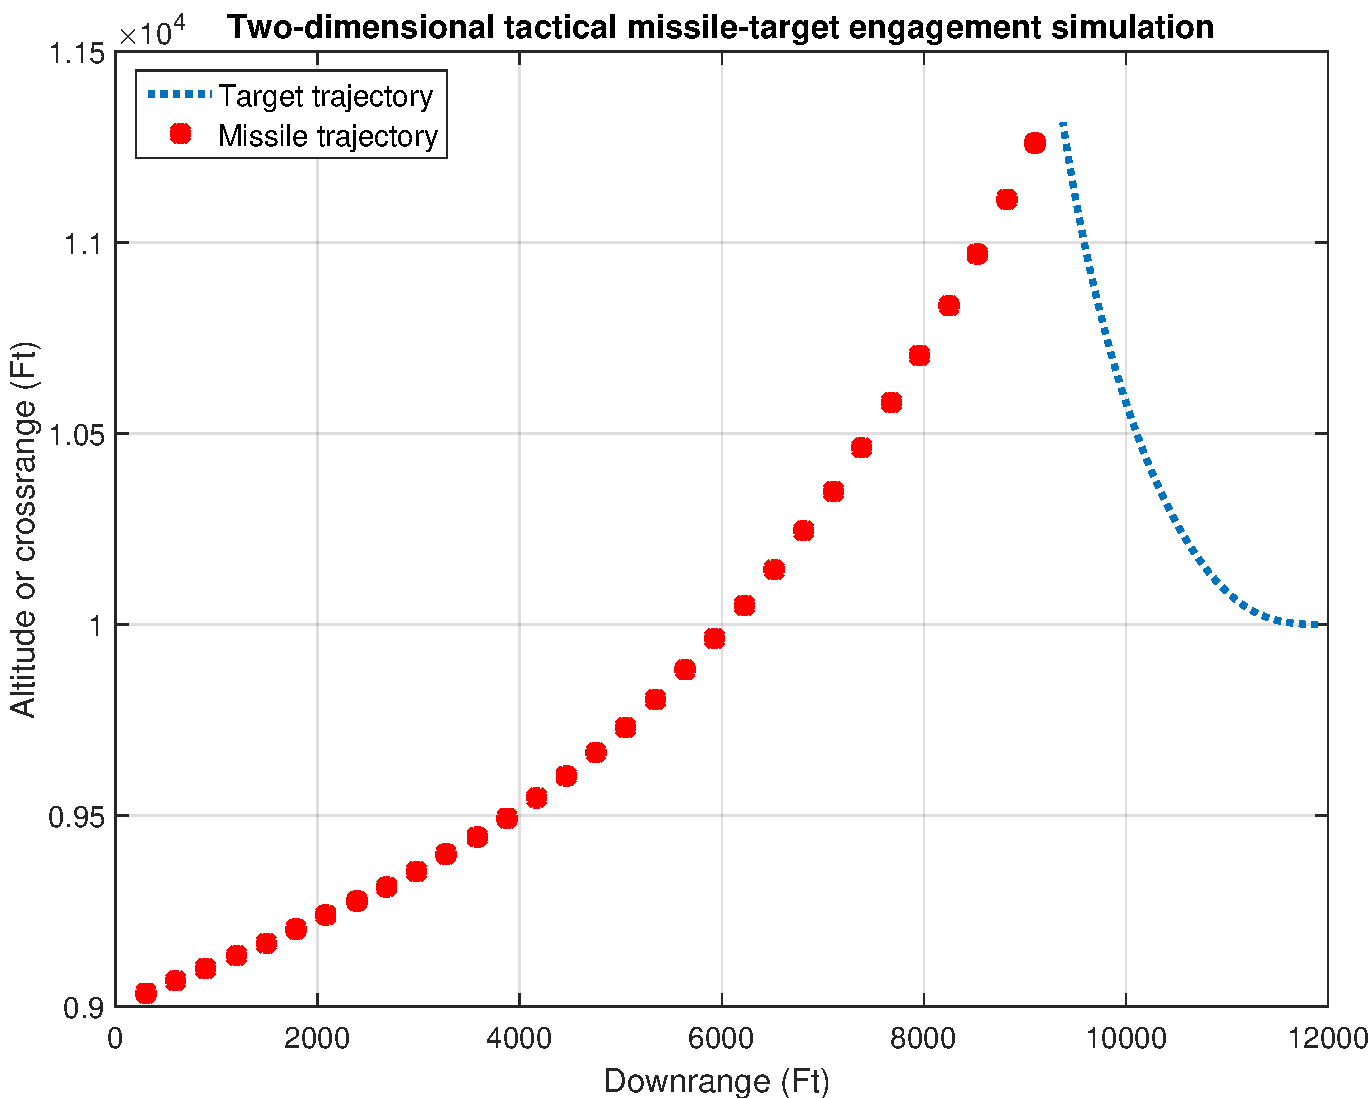
\includegraphics[scale = 0.75]{fig/trajectoryT1.pdf}
	\caption{Trajectory of the target and attacker in case of time at the end of the descent for the trapezoidal is equal to 8 }
	\label{trajectoryT1}
\end{figure}


\begin{figure}[htb]
	\centering
	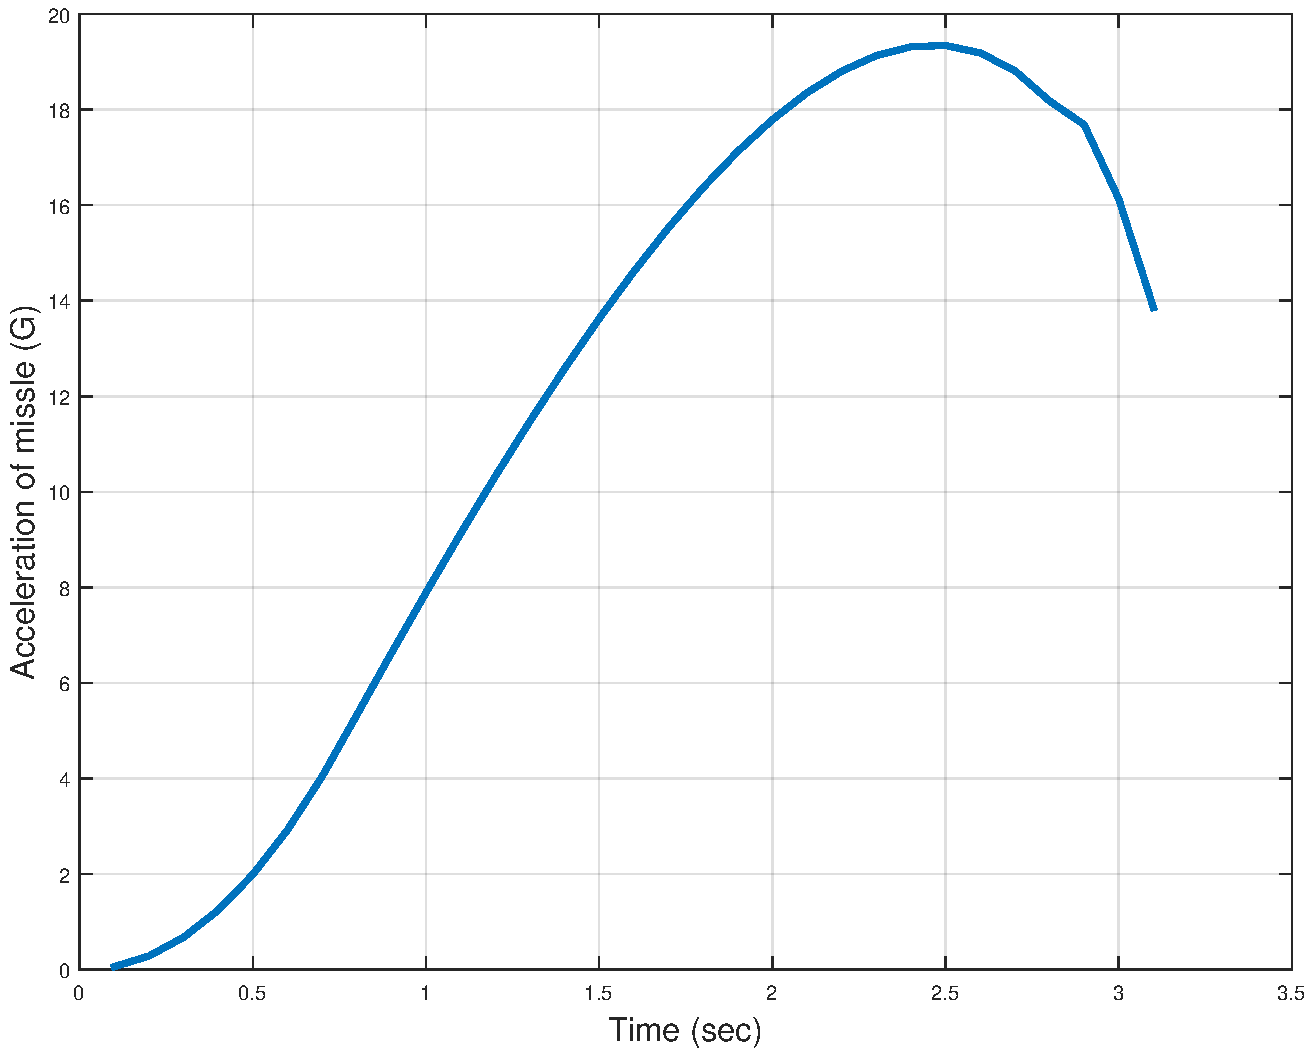
\includegraphics[scale = 0.75]{fig/MissileAccelerationT1.pdf}
	\caption{Missile acceleration in case of time at the end of the descent for the trapezoidal is equal to 8 }
	\label{missile accelerationT1}
\end{figure}

\begin{figure}[htb]
	\centering
	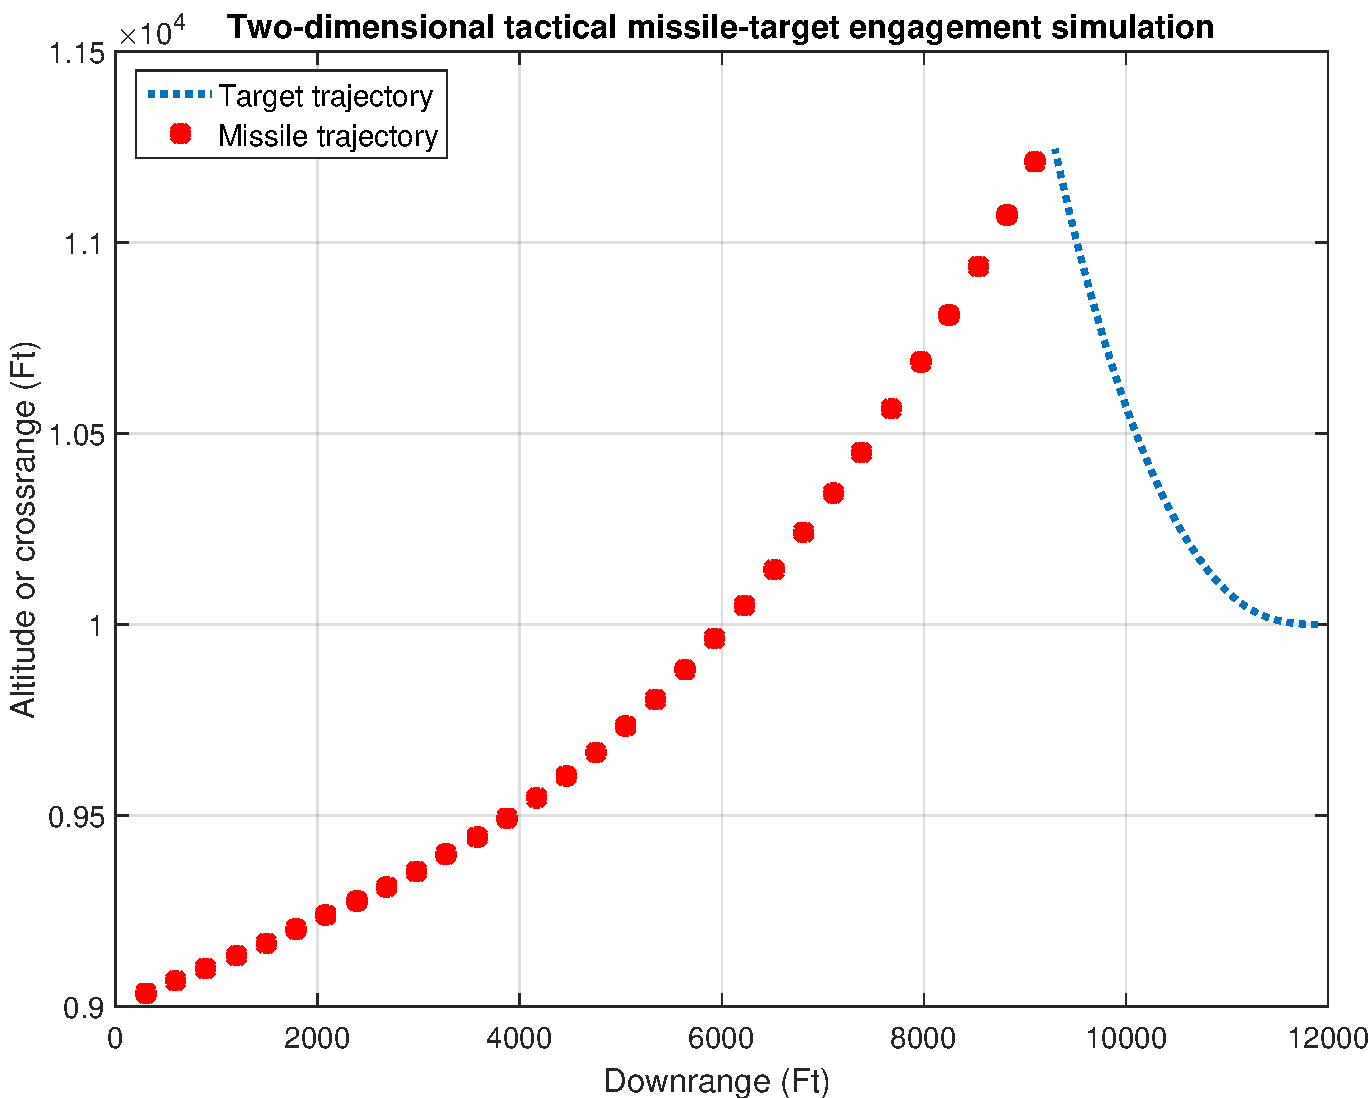
\includegraphics[scale = 0.75]{fig/trajectoryT2.pdf}
	\caption{Trajectory of the target and attacker in case of time at the end of the descent for the trapezoidal is equal to 5 }
	\label{trajectoryT2}
\end{figure}


\begin{figure}[htb]
	\centering
	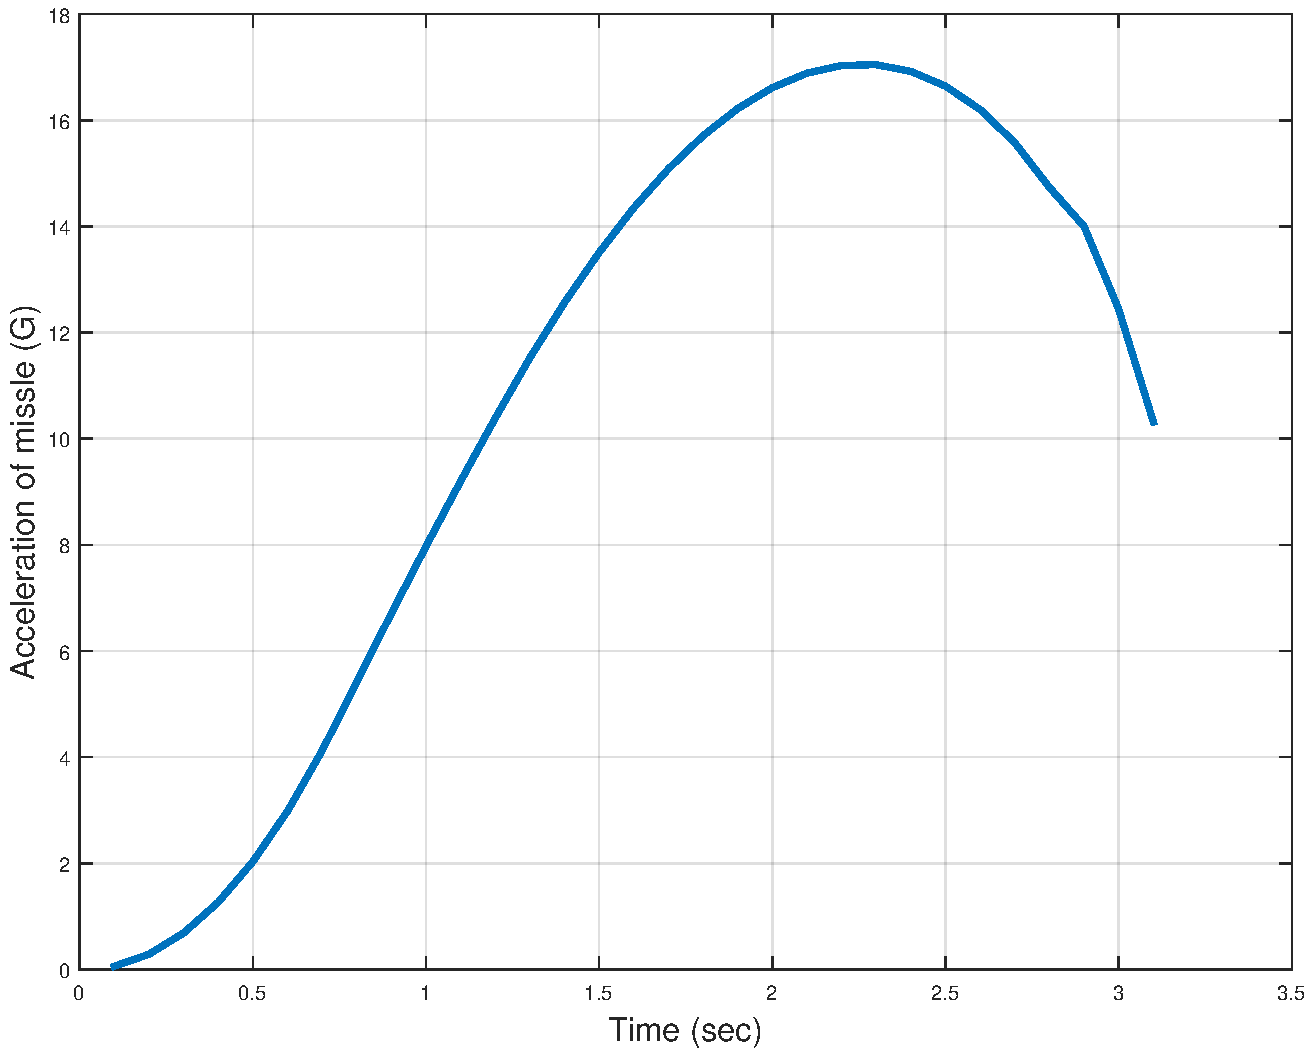
\includegraphics[scale = 0.75]{fig/MissileAccelerationT2.pdf}
	\caption{Missile acceleration in case of time at the end of the descent for the trapezoidal is equal to 5 }
	\label{missile accelerationT2}
\end{figure}


\begin{figure}[htb]
	\centering
	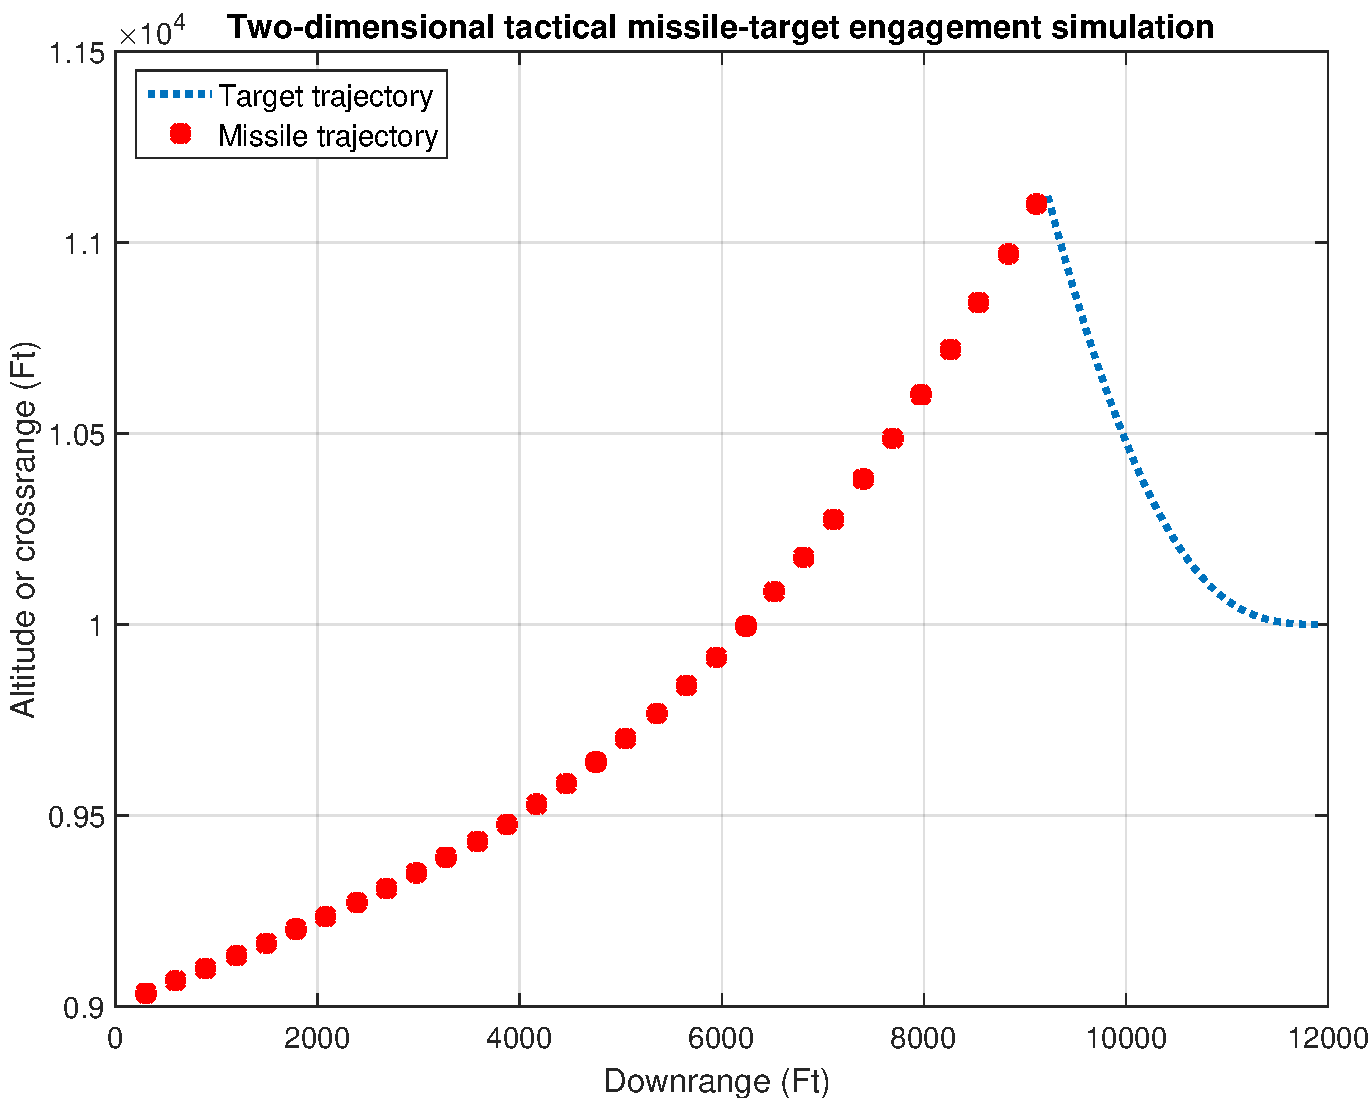
\includegraphics[scale = 0.75]{fig/trajectoryT3.pdf}
	\caption{Trajectory of the target and attacker in case of time at the end of the descent for the trapezoidal is equal to 4 }
	\label{trajectoryT3}
\end{figure}


\begin{figure}[htb]
	\centering
	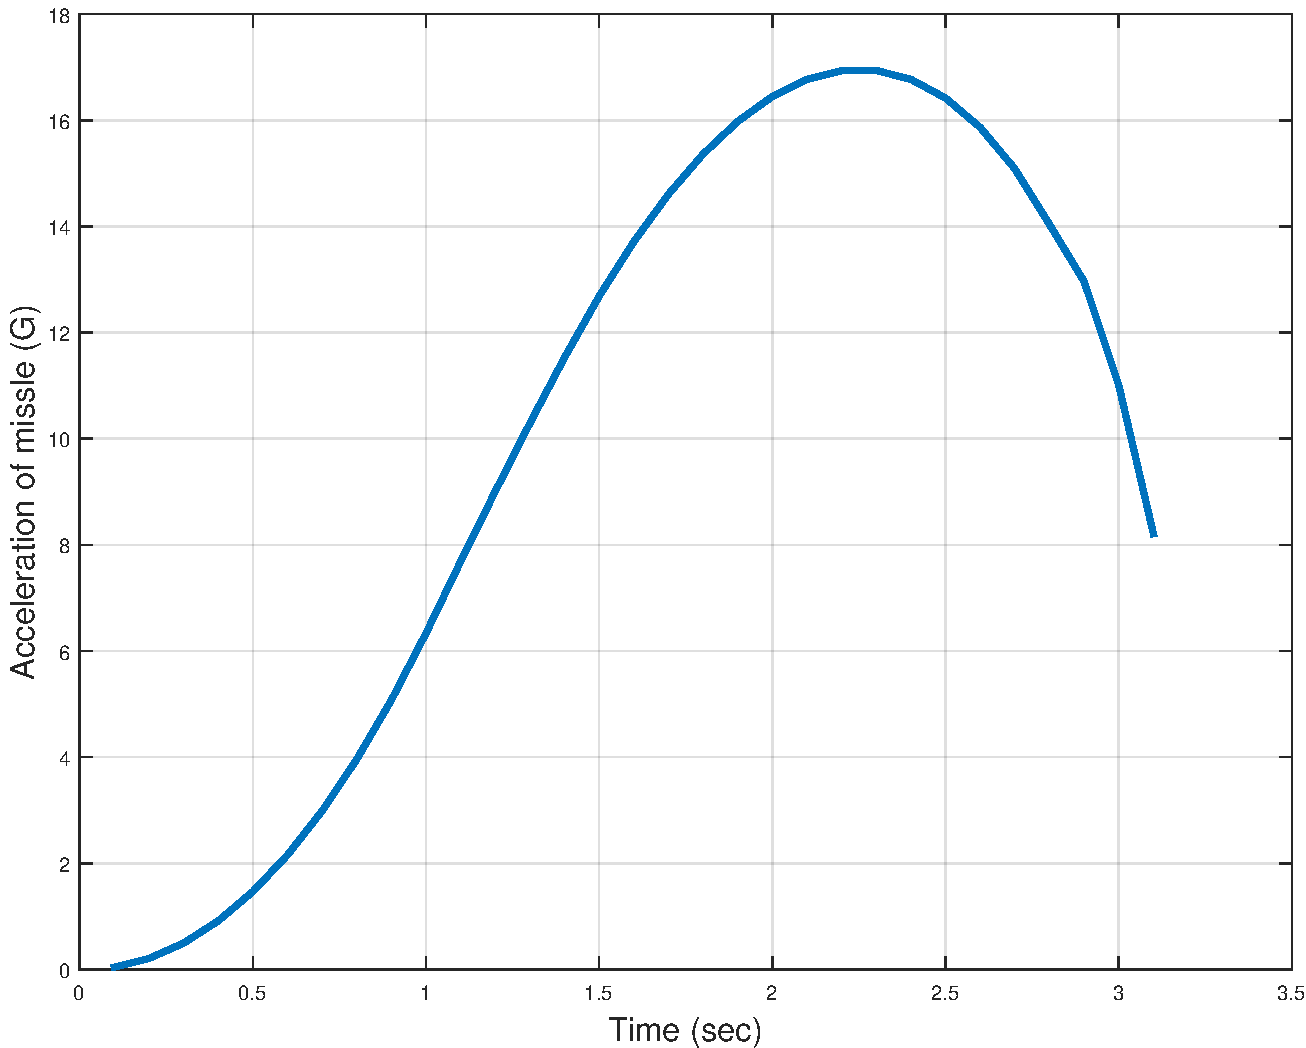
\includegraphics[scale = 0.75]{fig/MissileAccelerationT3.pdf}
	\caption{Missile acceleration in case of time at the end of the descent for the trapezoidal is equal to 4 }
	\label{missile accelerationT3}
\end{figure}
%-----------------------------------------------------

\subsection{Simulink Models}

In this section we will use the power of blocks in Simulink to solve the differential equations in section 2.3 in an easy way (Fig. \ref{PN eq}). We will make these equations as a main block (Fig. \ref{PN main block}) and as we change the inputs, we get the same results. The advantage of using simulink is to use the main block with an alternative optimization technique (like genetic algorithms). 

\begin{landscape}
\begin{figure}[htb]
	\centering
	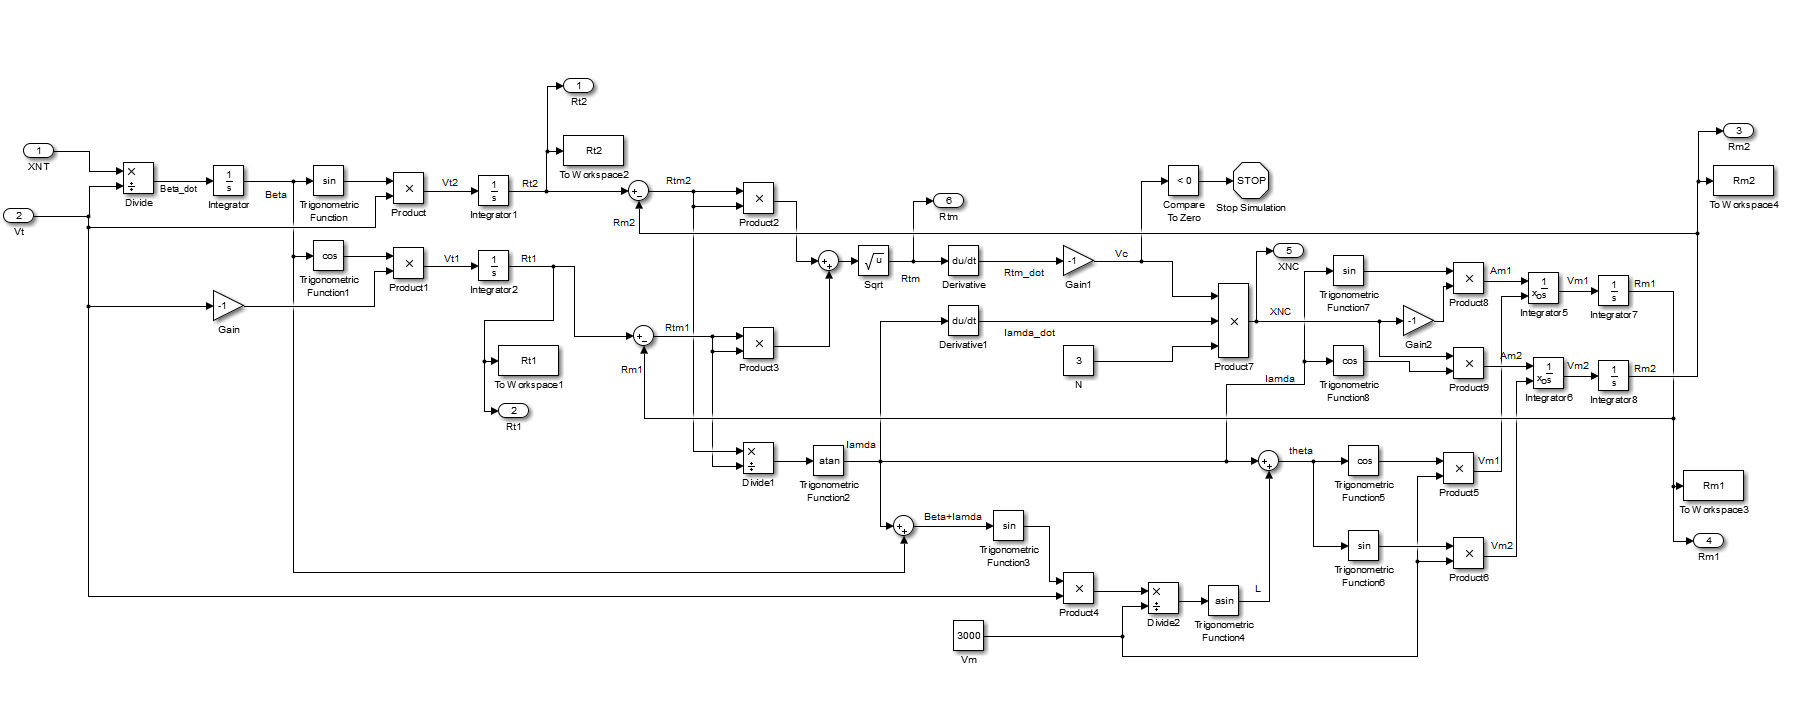
\includegraphics[scale = 0.70]{fig/PNeq.PNG}
	\caption{The Simulink model for proportional navigation equations in sec 2.3}
	\label{PN eq}
\end{figure}
\end{landscape}


\begin{figure}[htb]
	\centering
	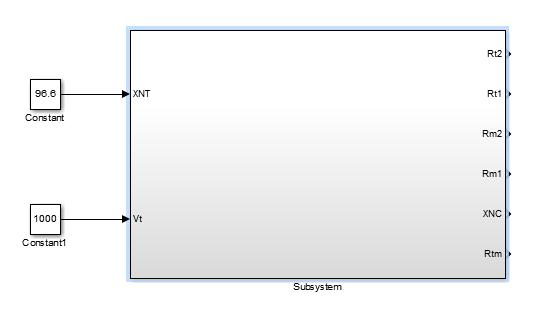
\includegraphics[scale = 0.75]{fig/PNmainBlock.PNG}
	\caption{The Simulink main block for solving proportional navigation equations in sec 2.3}
	\label{PN main block}
\end{figure}


% ===================================================
\section{Genetic Algorithms Solution}
We will use the main block we have created with the genetic algorithm toolbox in MATLAB in the same manner we have done, let the target maneuver ba a polynomial with unknown coefficients, then it is required to find the values of these coefficients using genetic algorithm to maximize miss distance and missile acceleration.


>>> long time for calculations

>>> if we changed some parameters in genetic ??!!
% ===================================================

% ===================================================
\section{Neural Networks Solution}
% ===================================================